% -*- Mode:TeX -*-

%% IMPORTANT: The official thesis specifications are available at:
%%            http://libraries.mit.edu/archives/thesis-specs/
%%
%%            Please verify your thesis' formatting and copyright
%%            assignment before submission.  If you notice any
%%            discrepancies between these templates and the 
%%            MIT Libraries' specs, please let us know
%%            by e-mailing thesis@mit.edu

%% The documentclass options along with the pagestyle can be used to generate
%% a technical report, a draft copy, or a regular thesis.  You may need to
%% re-specify the pagestyle after you \include  cover.tex.  For more
%% information, see the first few lines of mitthesis.cls. 

%\documentclass[12pt,vi,twoside]{mitthesis}
%%
%%  If you want your thesis copyright to you instead of MIT, use the
%%  ``vi'' option, as above.
%%
%\documentclass[12pt,twoside,leftblank]{mitthesis}
%%
%% If you want blank pages before new chapters to be labelled ``This
%% Page Intentionally Left Blank'', use the ``leftblank'' option, as
%% above. 

\documentclass[12pt,leftblank]{mitthesis}

\usepackage{lgrind}
%% These have been added at the request of the MIT Libraries, because
%% some PDF conversions mess up the ligatures.  -LB, 1/22/2014
\usepackage{cmap}
\usepackage[T1]{fontenc}
\pagestyle{plain} 

\usepackage{graphicx}
\graphicspath{ {images/} }
%% hehe.
\usepackage{coloremoji}

%% Little Essentials I'm adding
\usepackage{url} 
\usepackage{multicol}
\usepackage{array}
%%%%%%%%%%%%%%%%%%%%%%%%%%%%%%%


%% This bit allows you to either specify only the files which you wish to
%% process, or `all' to process all files which you \include.
%% Krishna Sethuraman (1990).

\typein [\files]{Enter file names to process, (chap1,chap2 ...), or `all' to
process all files:}
\def\all{all}
\ifx\files\all \typeout{Including all files.} \else \typeout{Including only \files.} \includeonly{\files} \fi

\begin{document}

% -*-latex-*-
% 
% For questions, comments, concerns or complaints:
% thesis@mit.edu
% 
%
% $Log: cover.tex,v $
% Revision 1.8  2008/05/13 15:02:15  jdreed
% Degree month is June, not May.  Added note about prevdegrees.
% Arthur Smith's title updated
%
% Revision 1.7  2001/02/08 18:53:16  boojum
% changed some \newpages to \cleardoublepages
%
% Revision 1.6  1999/10/21 14:49:31  boojum
% changed comment referring to documentstyle
%
% Revision 1.5  1999/10/21 14:39:04  boojum
% *** empty log message ***
%
% Revision 1.4  1997/04/18  17:54:10  othomas
% added page numbers on abstract and cover, and made 1 abstract
% page the default rather than 2.  (anne hunter tells me this
% is the new institute standard.)
%
% Revision 1.4  1997/04/18  17:54:10  othomas
% added page numbers on abstract and cover, and made 1 abstract
% page the default rather than 2.  (anne hunter tells me this
% is the new institute standard.)
%
% Revision 1.3  93/05/17  17:06:29  starflt
% Added acknowledgements section (suggested by tompalka)
% 
% Revision 1.2  92/04/22  13:13:13  epeisach
% Fixes for 1991 course 6 requirements
% Phrase "and to grant others the right to do so" has been added to 
% permission clause
% Second copy of abstract is not counted as separate pages so numbering works
% out
% 
% Revision 1.1  92/04/22  13:08:20  epeisach

% NOTE:
% These templates make an effort to conform to the MIT Thesis specifications,
% however the specifications can change.  We recommend that you verify the
% layout of your title page with your thesis advisor and/or the MIT 
% Libraries before printing your final copy.
\title{Reading Between the (Party) Lines: \\ \emph{An Analysis of Media Trust}}

\author{Sophie Beiying Chou}
% If you wish to list your previous degrees on the cover page, use the 
% previous degrees command:
%       \prevdegrees{A.A., Harvard University (1985)}
% You can use the \\ command to list multiple previous degrees
%       \prevdegrees{B.S., University of California (1978) \\
%                    S.M., Massachusetts Institute of Technology (1981)}
\department{MIT Media Lab}
\school{School of Architecture and Planning}

% If the thesis is for two degrees simultaneously, list them both
% separated by \and like this:
% \degree{Doctor of Philosophy \and Master of Science}
\degree{MS in Media Arts and Sciences}

% As of the 2007-08 academic year, valid degree months are September, 
% February, or June.  The default is June.
\degreemonth{June}
\degreeyear{2016}
\thesisdate{May 5, 2016}

%% By default, the thesis will be copyrighted to MIT.  If you need to copyright
%% the thesis to yourself, just specify the `vi' documentclass option.  If for
%% some reason you want to exactly specify the copyright notice text, you can
%% use the \copyrightnoticetext command.  
%\copyrightnoticetext{\copyright IBM, 1990.  Do not open till Xmas.}

% If there is more than one supervisor, use the \supervisor command
% once for each.
\supervisor{Deb Roy}{Associate Professor}

% This is the department committee chairman, not the thesis committee
% chairman.  You should replace this with your Department's Committee
% Chairman. 
\chairman{Pattie Maes}{Academic Head, Program in Media Arts and Sciences}

% Make the titlepage based on the above information.  If you need
% something special and can't use the standard form, you can specify
% the exact text of the titlepage yourself.  Put it in a titlepage
% environment and leave blank lines where you want vertical space.
% The spaces will be adjusted to fill the entire page.  The dotted
% lines for the signatures are made with the \signature command.
\maketitle

% The abstractpage environment sets up everything on the page except
% the text itself.  The title and other header material are put at the
% top of the page, and the supervisors are listed at the bottom.  A
% new page is begun both before and after.  Of course, an abstract may
% be more than one page itself.  If you need more control over the
% format of the page, you can use the abstract environment, which puts
% the word "Abstract" at the beginning and single spaces its text.

%% You can either \input (*not* \include) your abstract file, or you can put
%% the text of the abstract directly between the \begin{abstractpage} and
%% \end{abstractpage} commands.

% First copy: start a new page, and save the page number.
\cleardoublepage
% Uncomment the next line if you do NOT want a page number on your
% abstract and acknowledgments pages.
% \pagestyle{empty}
\setcounter{savepage}{\thepage}
\begin{abstractpage}
% this environment should probably be called abstract,
% but we want people to also be able to get at the more
% basic abstract environment
\def\abstractpage{\cleardoublepage
\begin{center}{\large{\bf \@title} \\
by \\
\@author \\[\baselineskip]}
\par
\def\baselinestretch{1}\@normalsize
Submitted to the \@department, \\
\@school \\
on \@thesisdate, in partial fulfillment of the \\
requirements for the \@degreeword\ of \\
\@degree
\end{center}
\par
\begin{abstract}}

TO-DO
\end{abstractpage}

% Additional copy: start a new page, and reset the page number.  This way,
% the second copy of the abstract is not counted as separate pages.
% Uncomment the next 6 lines if you need two copies of the abstract
% page.
% \setcounter{page}{\thesavepage}
% \begin{abstractpage}
% % this environment should probably be called abstract,
% but we want people to also be able to get at the more
% basic abstract environment
\def\abstractpage{\cleardoublepage
\begin{center}{\large{\bf \@title} \\
by \\
\@author \\[\baselineskip]}
\par
\def\baselinestretch{1}\@normalsize
Submitted to the \@department, \\
\@school \\
on \@thesisdate, in partial fulfillment of the \\
requirements for the \@degreeword\ of \\
\@degree
\end{center}
\par
\begin{abstract}}

TO-DO
% \end{abstractpage}

 

%%%%%%%%%%%%%%%%%%%%%%%%%%%%%%%%%%%%%%%%%%%%%%%%%%%%%%%%%%%%%%%%%%%%%%
% -*-latex-*-

% Some departments (e.g. 5) require an additional signature page.  See
% signature.tex for more information and uncomment the following line if
% applicable.
% -*- Mode:TeX -*-
%
% Some departments (e.g. Chemistry) require an additional cover page
% with signatures of the thesis committee.  Please check with your
% thesis advisor or other appropriate person to determine if such a 
% page is required for your thesis.  
%
% If you choose not to use the "titlepage" environment, a \newpage
% commands, and several \vspace{\fill} commands may be necessary to
% achieve the required spacing.  The \signature command is defined in
% the "mitthesis" class
%
% The following sample appears courtesy of Ben Kaduk <kaduk@mit.edu> and
% was used in his June 2012 doctoral thesis in Chemistry. 

\begin{titlepage}
\begin{large}
The following people served as readers for this thesis:

\signature{Sepandar Kamvar}{Associate Professor of Media Arts and Sciences \\
   MIT Media Lab}

\signature{Iyad Rahwan}{Associate Professor of Media Arts and Sciences \\
   MIT Media Lab}
 
\end{large}
\end{titlepage}
 
\cleardoublepage

\section*{Acknowledgments}

Thank you famiry-- sister
Thank you Linda and Keira
Thank you Deb
Thank you Ethan
THANK YOU NATHAN, I DON'T KNOW HOW YOU DO IT ALL
Thank you readers
Thank you LSM
Thank you Heather
Thank you figure makers 
Thank you Ramesh



 
\section*{Acknowledgments}
% I have learned many things from writing this thesis. 
% % Although it has helped me grow enormously as a scientist, the most valuable lessons I take away with me are, as always, of people. 
 
% It has helped me grow enormously as a scientist. Yet exploring new theories, methods, and even disciplines were only a small part of the valuable lessons I take with me beyond these glass walls. For that, I have many people to credit:
 
This thesis was written by one but supported by many.

Thank you to my advisor, Prof. Deb Roy, for giving me this opportunity.\\
Thank you to my readers Prof. Sep Kamvar and Prof. Iyad Rahwan, for your input and time.

Thank you to Prof. Ethan Zuckerman, for volunteering your time, your guidance, and your heart. 

%Thank you to my colleagues at the Laboratory for Social Machines, who are as thoughtful and caring as they are talented. Special thanks to Soroush Vosoughi, Prashanth Vijayaraghavan, Martin Saveski, and Eric Chu their support in this thesis, both technically and emotionally.

Thank you to my LSM family, I could not have done this without you. Special thanks to Eric Chu, Soroush Vosoughi, Prashanth Vijayaraghavan, and Martin Saveski for their help in this thesis. Thank you so much to Amber Franey and Heather Pierce for everything you've done-- and then some.


Thank you to my lovely family: \\
My wonderful parents, for being the love I wish to see in the world;  \\
My sister Cleo Chou, for being my Number One fan.  \\
Thanks as well to Caroline Sonett, \\ 
for your great support in every aspect of my life.
  
Thank you to Ramesh Sridharan and William Li, for being my first and funniest friends and co-authors at MIT. Thank you to Carrie Cai for being an A+ inspiration.

Thank you Nathan Matias, for (always) being so helpful. Thank you Edmond Awad for the statistical guidance and sense of humor. 

%Thank you Heather Pierce and Amber Franey, without whom LSM would not function.  

Thank you Linda Peterson and Keira Horowitz, for keeping this crazy place running.

% Thank you to the wonderful, weird Media Lab community for being a constant source of inspiration.

And a thank you to all else who have shaped me indefinitely in the past two years.

 
%%% 1 - Pager
% Thank you to my advisor, Prof. Deb Roy, for giving me this opportunity.\\
% Thank you to my readers Prof. Sep Kamvar and Prof. Iyad Rahwan, for your input and time.

% Thank you to Prof. Ethan Zuckerman, for volunteering your time, your guidance, and your heart. 

% Thank you to my colleagues at the Laboratory for Social Machines, who are as thoughtful and caring as they are talented. Special thanks to Soroush Vosoughi, Prashanth Vijayaraghavan, Martin Saveski, and Eric Chu their support in this thesis, both technically and emotionally.

% Thank you to my lovely family: \\
% My wonderful parents, for being the love I wish to see in the world;  \\
% My sister Cleo Chou, for being my Number One fan.  \\
% Thanks as well to Caroline Sonett, \\ 
% for your great support in every aspect of my life.
  
% Thank you to Ramesh Sridharan and William Li, for being my first and funniest friends and co-authors at MIT. Thank you to Carrie Cai for the laughter and support.

% Thank you Nathan Matias, for (always) being so helpful. Thank you Edmond Awad for the statistical guidance and sense of humor. 

% Thank you Heather Pierce and Amber Franey, without whom LSM would not function.  

% Thank you Linda Peterson and Keira Horowitz, for keeping this crazy place running.

% And a thank you to all else who have shaped me indefinitely in the past two years.


 
\afterpage{\blankpage}




\pagestyle{plain}
  % -*- Mode:TeX -*-
%% This file simply contains the commands that actually generate the table of
%% contents and lists of figures and tables.  You can omit any or all of
%% these files by simply taking out the appropriate command.  For more
%% information on these files, see appendix C.3.3 of the LaTeX manual. 
\tableofcontents
%\newpage 
\afterpage{\blankpage}
%\listoffigures
%\newpage
%\listoftables


\part{Small Data}
%% This is an example first chapter.  You should put chapter/appendix that you
%% write into a separate file, and add a line \include{yourfilename} to
%% main.tex, where `yourfilename.tex' is the name of the chapter/appendix file.
%% You can process specific files by typing their names in at the 
%% \files=
%% prompt when you run the file main.tex through LaTeX.

\chapter{Introduction} 

Does anyone trust the news anymore? Not according to the latest Gallup Poll, which showed that only 4 in 10 Americans believe that mass media does a good job of reporting the news ``fully, fairly, and accurately.'' It's a major decline since the survey was first taken in 1999, back when more than half (55\%) of Americans believed the news was trustworthy.

And the trend has been steadily downward: in short, the majority of Americans have had little to no trust in mass media news coverage since 2007: a discouraging view for a tumultuous time in journalism \cite{Gallup-trust-2015}.

But beyond frustrated readers and reporters, why does distrust in the news matter? For one, media bias---or at the very least, the \emph{belief of} a biased media bias---may have a significant impact on the practice of democracy. A 2006 study from Georgetown University shows that those with more negative attitudes towards the news tend to be more highly influenced by their partisan prior beliefs and less by contemporary issues and messages when voting \cite{ladd2005attitudes}. This implies that distrust of media plays a potential role in the polarization of American politics.

Additionally, our reactions to news stories-- as well as politics at large-- are largely driven by emotion. Historical trends, as well as present-day models, show a process largely influenced by feelings rather than facts.


In light of the upcoming 2016 elections, Part I explores perceptions of media trust in coverage of the presidential candidates. Claims of media bias and favoritism are especially high-stakes in election years, where trust has been shown to plummet \cite{Gallup-trust-2015}.  

We begin by examining some of the factors that contribute to the perception of media bias. In particular, how does the \emph{content} of a story (reading level and vocabulary) affect the reader versus the \emph{context} (source)? Although studies have been conducted to both examine the psychological effect of wording on believability and the impact of media brands and bias, separating and comparing these two factors remains largely unexamined \cite{weisberg2008seductive, baum2008eye}

To test our hypotheses on news trust, we perform a study on the crowdsourcing platform CrowdFlower. We manipulate the source of the story to examine effects of media brands on the reader, and also compare trust rankings between high and low reading level stories.


% From our findings in an experimental setting, we then extrapolate to another dimension of media: the social sphere of Twitter. In this dimension, we look for emotional signals in the text that cause it to become universally popular, with the goal of finding patterns cross party divides.

Although the general consensus of mistrust is clear, perception of media bias is a complex phenomenon to dissect, as it combines social and psychological effects with the traits of the story itself. This section hopes to shed light on some of these factors.

% This thesis hopes to shed new light on understanding what motivates readers' trust and distrust of news media, and pave pathways to understanding virality in the political news media. 
%   
\chapter{The Power of (Percieved) Media Bias}




\section{The Effects of Media Bias}

%Why is media bias IMPORTANT? Why is the problem IMPORTANT?

 
%- Fox News Effect
%- Does the media matter


\section{The Role of the Reader in Perceptions of Bias}

It comes as no surprise that our own political stances have a significant effect in our perceptions of bias in the media. 

In even seemingly neutral stories, partisans tend to view reporting as biased against their own views. This phenomenon---deemed the ``hostile media effect''---was first studied at Stanford University by Robert P. Vallone, Lee Ross, and Mark R. Lepper in 1985 \cite{vallone1985hostile}. Although ``true'' neutrality of a story is nearly impossible to quantify due to the subjective nature of the concept, Vallone et. al were able to successfully demonstrate that partisans of \emph{both} sides (pro-Israeli and pro-Arab) viewed the same news segments as hostile towards their beliefs and favorable to the other side.

%? Perceptions of media bias, then, have as much to do as self-serving motivations to secure preferential treatment as they do with the media itself.
  
%? The political leanings of the reader are essential considerations when attempting to measure other factors that contribute to bias. In 

\section{The Role of Media Brands in Perceptions of Bias}
%The media, of course, is not just one unified mass, and in an increasingly fragmented ecosystem, the role of media brands is a crucial factor in the perception of bias. Although most research
%\cite{baum2008eye}


 
%For instance, most research on the hostile media phenomenon conceptualizes the news media as an undifferentiated mass of information sources that individuals can (and do) reasonably characterize as having a uniform political orientation (Giner-Sorolla and Chaiken 1994, Peffley et al. 2001, Eveland and Shah 2003). Yet, the past two decades have seen a dramatic increase in the number and variety of news sources. One consequence is that Democrats and Republicans are increasingly likely to differ systematically in their assessments of specific media outlets.






%With the decline of print newspapers, a diverse number of new platforms and web-centric publications have risen.


%How do you control for the above things in your study?

\section{The Role of Language [Policial Persuasion]}




\subsection{Language and Politics}
%Presidential speeches degrading over time-- ie simple language appeals to the masses in politics
\subsection{The Seductive Allure [... of Simple] Language}
%But we trust complex language for explaining technical facts

%Test image

%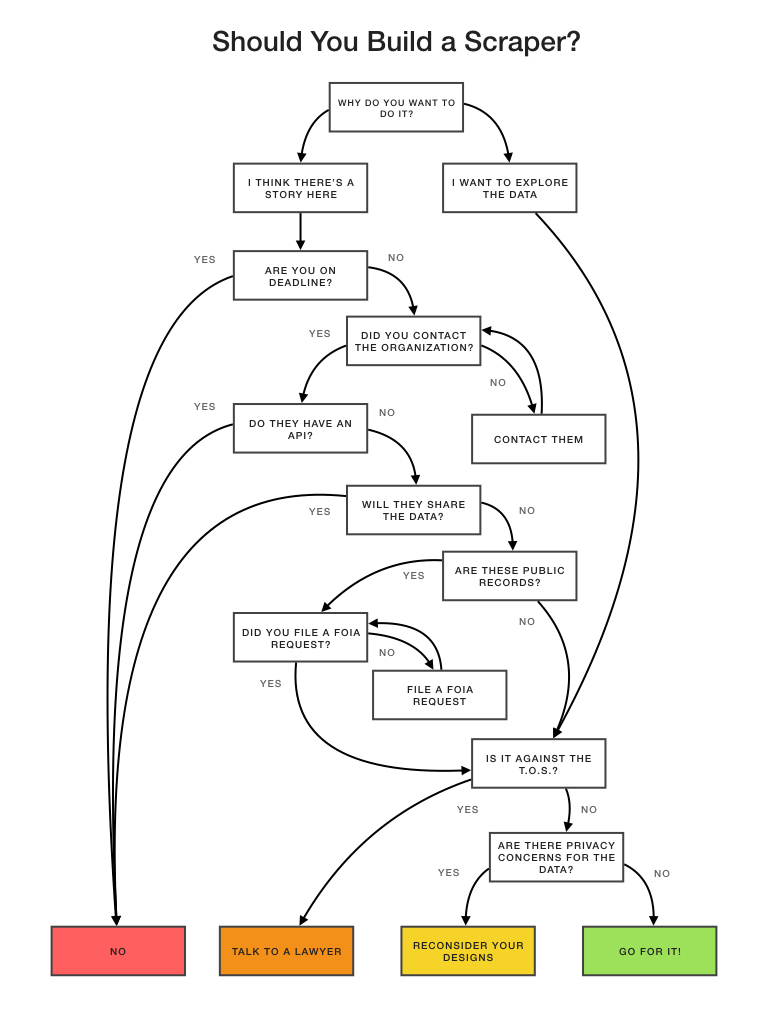
\includegraphics[width=\textwidth]{flowchart_final}


\section{Importance in Political Outcomes}
%Fox news effect 

\section{The 2016 Elections} 
\subsection{Criticism of Media Bias} 
%(Obama Speech)

%So.... are you what you cover?









\chapter{Data Collection}

\section{The Electome}

The Electome is a large, collaborative, and ongoing effort in the Laboratory for Social Machines that seeks to analyze the ``competition of ideas'' in the upcoming 2016 elections. It does so by using techniques in natural language processing, machine learning, and network analysis to make sense of ``big data'' collected from two main sources: traditional media (online versions of news publications) and social media (Twitter) \cite{vvr_electome2016}. 

This thesis, which emerged from the Electome, examines a narrowed portion of the first dataset centered around specific topics and candidates. The following section will describe the methods used to gather this dataset as well as shared machine learning tools for article classification.

\section{Story Collection} 

News articles from 14 different news publications were systematically collected every hour from RSS feeds beginning from January 2015. The outlets tracked are:
 

\begin{multicols}{2}
    \begin{itemize}
    \itemsep-1em 
      \item CNN
      \item Fox News
      \item The Wall Street Journal
      \item ProPublica
      \item Politico
      \item McClatchy
      \item The Washington Post
      \item Buzzfeed (News only)
      \item National Public Radio (NPR)
      \item The Huffington Post
      \item The Associated Press
      \item Reuters
      \item The New York Times
      \item The Los Angeles Times
    \end{itemize}
\end{multicols}

The above outlets were chosen to form a diverse subset of the current U.S. news ecosytem, including a combination of private and public, liberal and conservative, legacy and new media publications. Also included are wire services and a mix of media delivery formats for which the outlet is known (radio, television, print, or web).

Steps to collect the news stories were as follows:

 \begin{enumerate}
    \item For each news publication:
    \begin {enumerate}
    \itemsep-1em 
        \item Use regular expressions to extract all RSS feed urls for a news site.
        \item For each RSS feed:
        \begin {enumerate}
        \itemsep-1em 
            \item Parse feed using open source xml reader library, Feedparser.
            \item For each link to a story in the feed:             
            \begin {enumerate}
                \item Parse html using Beautiful Soup 3 (an open source python library)
                \item Insert headline, authors, story text, publication date and retrieval date into an SQL database.

            \end {enumerate}
        \end{enumerate}
    \end{enumerate}
\end{enumerate}

Data depulication (by story url and headline) is then performed to ensure only one copy of each article is in the database. This step is necessary as articles from wire services often appear across many outlets and effect aggregate text analsyis.

On average, 2,000 stories are collected per day across all outlets. However, volume follows a consistent pattern of fluctuation depending on weekday, ranging from approximately 1,000 to 3,000 stories.

[INSERT HERE GRAPH OF NEWS STORIES VOLUME BY WEEKDAY]

As of March 1st, 2016, there were 855,000 stories collected in the database and 43,000 journalists.

For the purposes of this study, stories were examined from five outlets: 

\begin{itemize}
\itemsep-1em 
  \item CNN
  \item Fox News  
  \item The New York Times
  \item The Wall Street Journal 
  \item The Associated Press 
\end{itemize}

The choices consist of two pairs of outlets in both print and television across the liberal-conservative divide, plus a wire service. Of the 14 outlets above, both Fox News and the Wall Street Journal have an audience that leans conservative compared to the overall population (27\% mostly conservative viewers versus 17\% in the overall population for Fox News and 22\% mostly conservative viewers versus 17\% in the overall population) measured by a 2014 Pew survey \cite{PoliticalPolarization}.

On the other hand, the New York Times and CNN both have audiences that lean mostly liberal (25\% liberal versus 22\% in all respondents for CNN and 25\% for the New York Times). The Associated Press, which was not included in the survey, has members in outlets across the political divide and was chosen as an experimental control.
 
For further analysis, see section 4.1.

\section[Election Classification] {Election Classification\footnote{footnote}}

[How do I cite Prashanth's unpublished work?]
 

Election Classifier
The election classifier is a binary classifier which takes a news article as input and determines whether it is about the 2016 US election or not. Since news articles usually contain clean and structured language, they can easily be classi- fied as election-related using Bag-of-Word (BoWs) features. We used the chi-square test for feature selection. Chi-square measures the lack of independence between a term in an article and a class (in this case the election). High scores on chi-square indicate that the null hypothesis of independence should be rejected and thus that the occurrence of the term and class are dependent. The features are ranked based on their scores and the top 20,000 features form the vocabulary for the binary classifier. Next, using scikit-learn (Pedregosa et al. 2011)–a Python machine learning library– a binary Maximum Entropy (MaxEnt) text classifier (Nigam, Laf- ferty, and McCallum 1999) is trained on a balanced dataset of 1,000 manually labelled news articles. The classifier was evaluated on a separate balanced test set of 300 articles, with the precision and recall of the election-related articles being 0.9 and 0.91 respectively (F-score of 0.92).
Figure 6 shows the number of election-related articles, ag- gregated weekly from February 2015 to December 2015 (to- tal of 38,595 election-related articles). As was the case with Twitter, the number of election-related articles increase as we get closer to the election. All election-related articles are next passed to three classifiers: topic, sentiment and candi- date.

\section[Topic Classification] {Topic Classification\footnote{footnote}}
[How do I cite Prashanth's unpublished work?]
 

\begin{multicols}{2}
    \begin{itemize}
    \itemsep-1em 
      \item Income Inequality
      \item Environment/Energy
      \item Jobs/Employment
      \item Guns
      \item Racial Issues
      \item Foreign Policy/National Security
      \item LGBT Issues
      \item Ethics
      \item Education
      \item Financial Regulation
      \item Budget/Taxation
      \item Veterans
      \item Campaign Finance
      \item Surveillance/Privacy
      \item Drugs
      \item Justice
      \item Abortion
      \item Immigration
      \item Trade
      \item Health Care
      \item Economy
      \item Other 
    \end{itemize}
\end{multicols}
 


\section{Flesch-Kincaid Readability Tests} 
In this study, we focus primarily on the Flesch-Kincaid (F-K) tests for estimating text readability. Originally developed for the U.S. Navy in 1975 for assessing the difficulty of technical manuals, the F-K reading level corresponds roughly to U.S. grade level and the reading ease score is inversely proportional to the grade level on a scale from 0 to approximately 120 \cite{kincaid1975derivation}.

We chose the F-K tests over other comparable ones due to its popularity in educational assessment and other applications, including in legislation. For example, it is required by law in Florida that life insurance policies have a Flesch reading ease of 45 or greater (less than 12th grade in reading level) \cite{Statu37online}. The F-K tests are also bundled in many common word processing services, including Microsoft Office Word. As a comparison, basic article analysis is also computed using the Gunning fog index (see Section 5.2.1).

The formula for Flesch reading ease is as follows:

$$206.835 - 1.015 \left( \frac{\mbox{total words}}{\mbox{total sentences}} \right) - 84.6 \left( \frac{\mbox{total syllables}}{\mbox{total words}} \right)$$

And for reading grade level:

$$0.39 \left ( \frac{\mbox{total words}}{\mbox{total sentences}} \right ) + 11.8 \left ( \frac{\mbox{total syllables}}{\mbox{total words}} \right ) - 15.59$$
 
The two formulas are not directly comparable due to the difference in weighting factors. For ease of metaphor, we use the grade level tests in our analysis. Syllable length is highly weighted in this formula, so it is possible to generate a story of very high reading level that consists of a single word in a single sentence (the longest English word, \emph{pneumonoultramicroscopicsilicovolcanoconiosi}, a type of lung disease, has a reading grade level of 197.2), which is a limitation of the method, since texts with polysyllabic words are not always necessarily more difficult to read.
  
\chapter{Experimental Design}


\section {Data Selection} 

For this study, we chose to analyze stories collected between January 1, 2016 (the start of the election year) and March 1, 2016 (Super Tuesday). Since a large number of states hold primary elections and caucuses on Super Tuesday, it is seen as an early indicator of candidate electability. All stories had been filtered through both the election (see section 3.3) and topic (see section 3.4) classifiers.

Based on the results of Super Tuesday, we selected four candidates for this study by delegate count: Hillary Clinton (1,279), Bernie Sanders (1,027), Donald Trump (743), and Ted Cruz (517) \cite{March45online}.

News articles were then separated into single-candidate stories (i.e. articles featuring primarily one candidate in the headline) to be able to measure more clearly the percieved bias per candidate. This was done programatically using regular expressions to determine if a headline contained one candidate and one candidate only. A dictionary of related names was created to make sure that stories were correctly categorized (i.e. ``Hillary'', ``Clinton'', and ``Hillary Clinton'' were to be categorized as pertaining to ``Hillary Clinton'' but not if preceded by ``Bill'').

\subsection {Publication Selection}

For the purposes of this study, stories were examined from five outlets: 

\begin{itemize}
\itemsep-1em 
  \item CNN
  \item Fox News  
  \item The New York Times
  \item The Wall Street Journal 
  \item The Associated Press 
\end{itemize}

The choices consist of two pairs of outlets in both print and television across the liberal-conservative divide, plus a wire service. Of the 14 outlets above, both Fox News and the Wall Street Journal have an audience that leans conservative compared to the overall population (27\% mostly conservative viewers versus 17\% in the overall population for Fox News and 22\% mostly conservative viewers versus 17\% in the overall population) measured by a 2014 Pew survey \cite{PoliticalPolarization}.

On the other hand, the New York Times and CNN both have audiences that lean mostly liberal (25\% liberal versus 22\% in all respondents for CNN and 25\% for the New York Times). The Associated Press, which was not included in the survey, has members in outlets across the political divide and was chosen as an experimental control. 

[MIGHT INCLUDE THOSE DISTRIBUTIONS HERE]

\subsection {Topic Selection}


first show breakdowns

Immigration                         4
Abortion                            3
Campaign Finance                    2
Foreign Policy/National Security    1




Single top topic

SHOW THE TOPIC HISTOGRAMS
TO SHOW WHY YOU CHOOSE THOSE (LIMITING FACTOR)


\subsection {Flesch Kincaid Cutoffs}
\subsection {Redaction of Stories}

 

\section{CrowdFlower}
\section{Demographic Survey}
\section{Political Affiliation Survey}
\section{Quality Assurance}
%-Filter by nationality
%- highest setting on crowdflower
%- Gold questions
%- time limits
%- price
\chapter{Study}

\section{Motivations}

%From our exploratory study, we were able to obtain a significant but weak effect between disclosing the source and the levels of trust marked by readers towards an article.

% We also observed trends that suggested an interaction between disclosing the source and the reading level of a story.

% However, the study faced several limitations: first, we did not obtain enough samples to show a statistically significant result for interactions between source and reading level.

% Furthermore, multiple levels of independent variables (ie: 5 levels for input source) made modeling complex and the results less clear.

% The dataset was also unbalanced and sparse (ie, because of large numbers of input variables we did not have complete representation for each category, such as high, low, and mid-reading level stories for every outlet and topic). We tried to control for those factors by randomization, however it made more difficult to analyze specific correlations between source and trust.

% To further explore the interaction between disclosing the source and the reading level of the story, we set up another crowdsourcing experiment on CrowdFlower, this time targeting this specific interaction, to see if there is a significant effect between the two, detailed in the following chapter.
 
This study sets out to tackle the question of reading level's effect in perceptions of news bias. In particular, how does it compare to factors associated with latent biases of the reader, such as media brand?

Although the body of literature in Chapter 2 examines the theories behind partisanship and media branding, little work has been done to compare those contextual effects with the effects of \emph{content} within a story, such as language use.

This thesis tests six hypothesis.

We explore two novel hypotheses testing reading level effects:

\begin{itemize}
\item \textbf{H1}: High reading level stories increase trust in the story.
\item \textbf{H2}: However, they decrease perceptions of fairness. 
\end{itemize}

As well as two comparing the role of \emph{content} versus \emph{context}:

\begin{itemize}
\item \textbf{H3}: Media brand has a stronger role in determining story trust than the content. 
\item \textbf{H4}: Media brand has a stronger role in determining story fairness than the content.
\end{itemize}

And two verifying former theories:
\begin{itemize}
\item \textbf{H5}: Stories shown to be from outlets of aligned political party score significantly higher on both trust and fairness than those of the opposite.
\item \textbf{H6}: Stories about candidates opposite to the readers preferred candidate score significantly lower in fairness, regardless of outlet.
\end{itemize}

We hypothesis \textbf{H1}: that high reading level of stories increase trust based off the work from Weisberg et. al showing that neuroscience explanations sway believability of scientific explanations, due to the field-specific nature of political reporting \cite{weisberg2008seductive}.

Conversely, we predict \textbf{H2} that it creates a decrease in the perception of fairness in the story, due to the polarizing nature of political news and the fact that more complex stories could cause a partisan individual to more quickly reject what appears as an onslaught of conflicting information \cite{cacioppo1979effects}.
 
 We hypothesize \textbf{H3} and \textbf{H4} that media brand effects outweigh content in determining both trust and fairness.

 Finally, we expect to see hostile media effects (\textbf{H5} and \textbf{H6}) to emerge.

\section{Experimental Design}
%For the second study, our experiment was revised to have a 4 x 2 mixed-factorial design.
Our experiment has a 4 x 2 mixed-factorial design.
 
\begin{center}
\begin{table}
\begin{tabular}{ | m{5em} | m{7em}| m{7em} | m{7em} | m{7em} | } 
 \hline
  & \textbf{Source: None} & \textbf{Source: AP} & \textbf{Source: Fox} & \textbf{Source: CNN} \\
 \hline
 \textbf{High Reading Level} & Clinton, Cruz, Sanders, Trump & Clinton, Cruz, Sanders, Trump & Clinton, Cruz, Sanders, Trump & Clinton, Cruz, Sanders, Trump  \\ 
 \textbf{Low Reading Level} & Clinton, Cruz, Sanders, Trump & Clinton, Cruz, Sanders, Trump & Clinton, Cruz, Sanders, Trump & Clinton, Cruz, Sanders, Trump \\ 
 \hline
\end{tabular}
\caption{Main Study Design}
\label{study2}
\end{table}
\end{center}
\newpage

% \begin{itemize}
%   \item Source (4 levels: None, AP, CNN, Fox)
%   \item Candidate (4 levels: Clinton, Cruz, Sanders, Trump)
%   \item Reading Level (2 levels: High, Low)
% \end{itemize}

In this study, reading level of articles and candidates featured in the articles were treated as within-subject variables, and the source of the story between-subjects.

% This time, we reduced the number of stories to N=8, and also changed reading level from a 3-level to 2-level variable (low, high) for clarity.

% Most significantly, since we observed some significant effect from disclosing source to the reader in Study 1, we added a manipulation in this experiment to further study the effect of revealing the source:

% Following Baum's research in showing the effects of media brands and reader bias by manipulating reported brands, all eight stories in Study 2 were in fact written by the Associated Press, however, we manipulated the source shown to the reader \cite{baum2008eye}. In group A, readers were shown the headline and text of the story with no other context. In group B, readers were additionally shown that the story was from the Associated Press (true label). In groups C and D, readers were shown that the story was from CNN and Fox News, respectively.

Each participant reads eight stories, two each of high and low reading level per candidate. However, to examine effects of media brands and reader bias, we manipulate the source attributed to the story, building off Baum's research in media brands and television reporting \cite{baum2008eye}.

All eight stories in Study 2 were in fact written by the Associated Press, however, readers are divided into four groups receiving different labels. In group A, readers were shown the headline and text of the story with no other context. In group B, readers were additionally shown that the story was from the Associated Press (true label). In groups C and D, readers were shown that the story was from CNN and Fox News, respectively.

This setup was created to eliminate some of the confounding effects from using stories from different sources (writing style, focus of content, slant, etc.), while directly observing the effect of revealing a specific source to the reader. The Associated Press was chosen as the source of the stories as it is the highest circulation newswire service in the United States, and has 14,000 members that use its content \cite{apFAQ}. Notably, both CNN and Fox News publish content in full or part from the Associated Press, although the specific stories chosen had not been published in full by either to avoid bias.

After each article, we ask the reader to rank the fairness of the story on a 5-point Likert scale as well as its truthworthiness.

\subsection{Dataset} 
Eight stories were chosen for this study: two (high and low reading level) per candidate. All eight stories were written by reporters from the Associated Press (although they may have been republished elsewhere).

Reading level cutoffs were made by taking the bottom and top 25\% percentile of Flesch-Kincaid scores for each candidate. From stories written by the Associated Press that made the cutoff, we formed pairs of high and low reading level stories from each topic. The topic with the highest distance between reading level in the pair was chosen for each candidate.

% put histograms of reading level with cutoff lines
 
\subsection{Survey Design}
We designed four surveys (1 per group) on the platform CrowdFlower. Each participant was randomnly assigned to a group and could not take the survey more than once. The eight stories were shown (in a randomized order), and each story was followed up by two scoring questions pertaining to fairness and trustworthiness.

\begin{figure}[H] 
\centering
  \frame{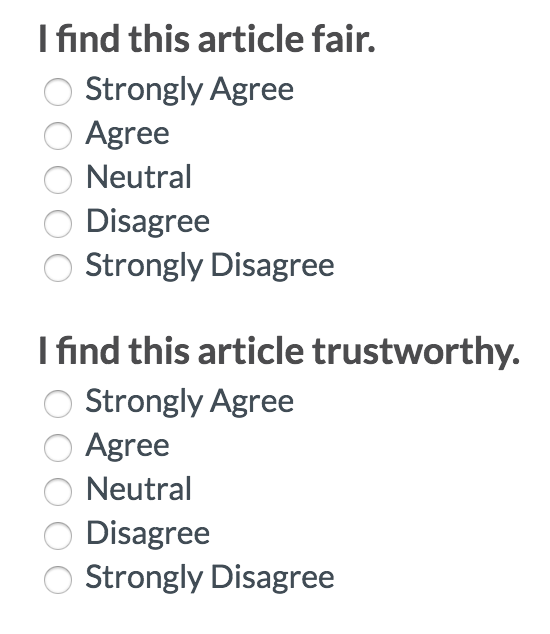
\includegraphics[width=0.45\textwidth]{study2_qs}}
  \caption{Scoring Questions for Survey}
\end{figure}

The survey concluded with an abbreviated standard demographic survey as well as a political affiliation survey adapted from Pew's standard polling survey \cite{Pew-demographics}. These more personal questions were placed at the end to prevent priming readers beforehand.


\begin{figure}[h!] 
\centering
  \frame{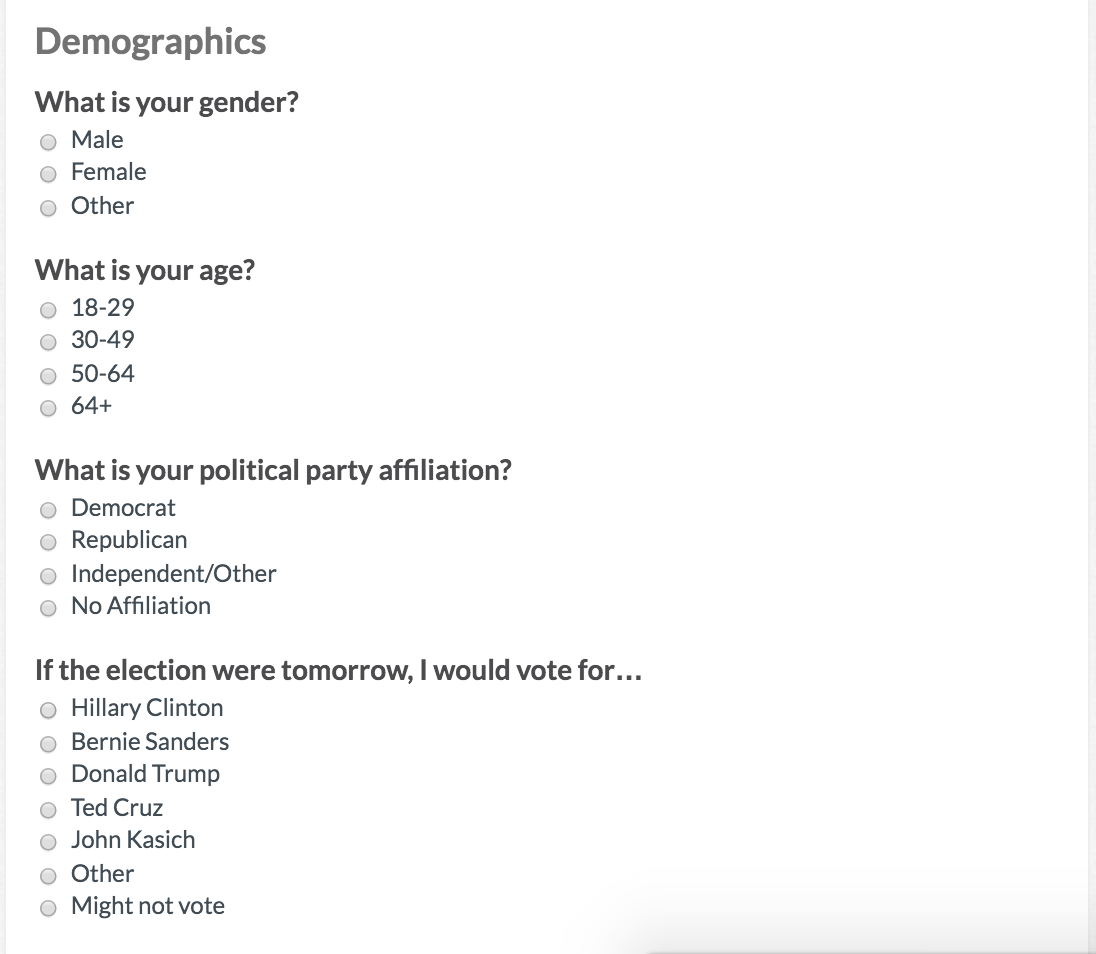
\includegraphics[width=0.45\textwidth]{demographic_qs}}
  \caption{Demographic Questions for Survey}
\end{figure}

Finally, we asked readers to report whether or not they migh have read the stories before.

\begin{figure}[H] 
\centering
  \frame{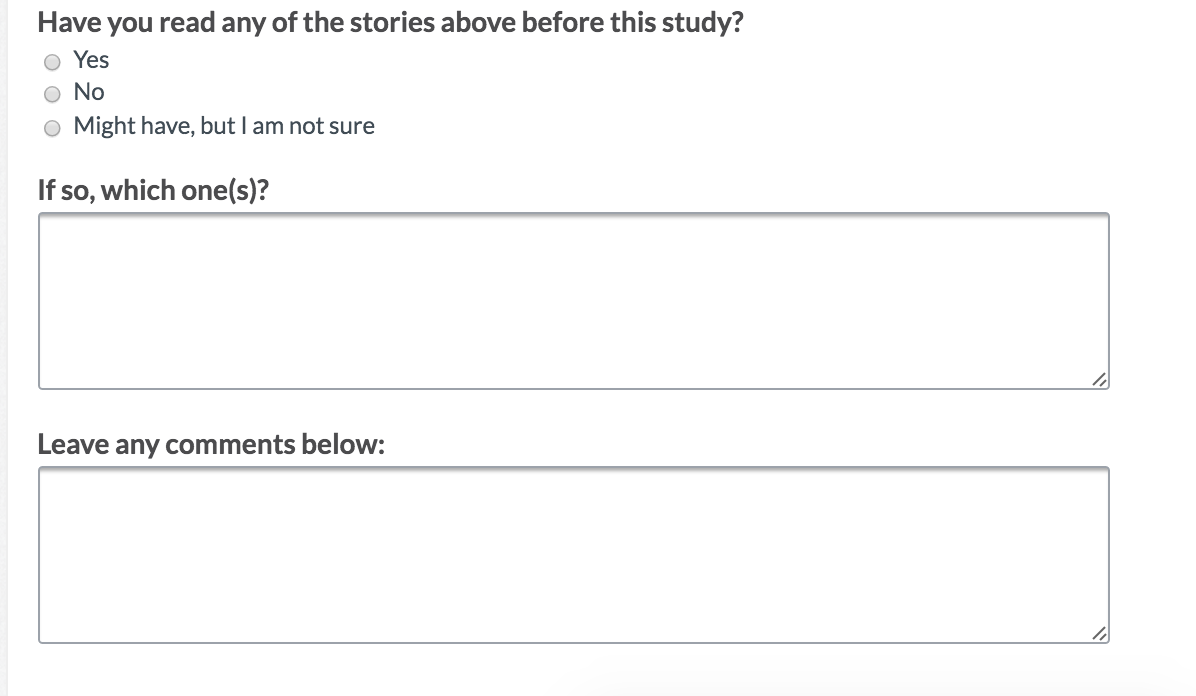
\includegraphics[width=0.45\textwidth]{survey_comments}}
  \caption{Comments for Survey}
\end{figure}

We ran the survey of a duration of  hours and had 40 participants sign up per group, for a total of 160 participants.

\subsection{Quality Control}

CrowdFlower has a built-in ``Test Question'' feature that allows for the rejection of a annotator whose answers to specific questions do not lie within a threshold (default 70\%) of the ``correct'' answer or whose answers lay outside the standard variation compared to others.

However, since the questions we asked were by nature subjective and therefore outliers and disagreements in answers could imply signal rather than noise, we chose to monitor for quality using other metrics instead. CrowdFlower was not designed explicitly for survey-like tasks, and therefore there were no options for different screening methods or questions. Gold Questions on the platform are selected by the creator within the set of all questions being recorded.

Because of this, we monitored quality of results in two ways:

First, by setting a minimum of time of 360 seconds to complete the task of reading 5 stories for a task to be accepted.

Second, by selecting only Level 3 contributors on CrowdFlower as suggested on their website for handling survey-like tasks \cite{CrowdFlower-guide}.

Level 3 contributors are described as those who ``have completed over a hundred Test Questions across hundreds of different Job types, and have a near perfect overall Accuracy'' \cite{CrowdFlower-levels}. This is the highest category of contributor.
 
Users were also only allowed to answer the set of questions once. 

\$0.80 was given per survey, as suggested by MIT Committee on the Use of Humans as Experimental Subjects. The average response time per survey was 09:20 min.


\section{Basic Analysis}

\subsection{Demographics}

\begin{figure}[H] 
\centering 
  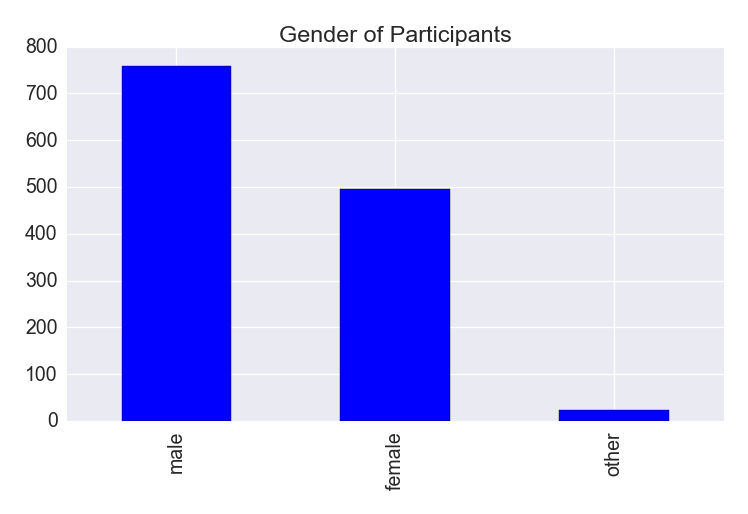
\includegraphics[width=0.49\textwidth]{gender_study2} 
  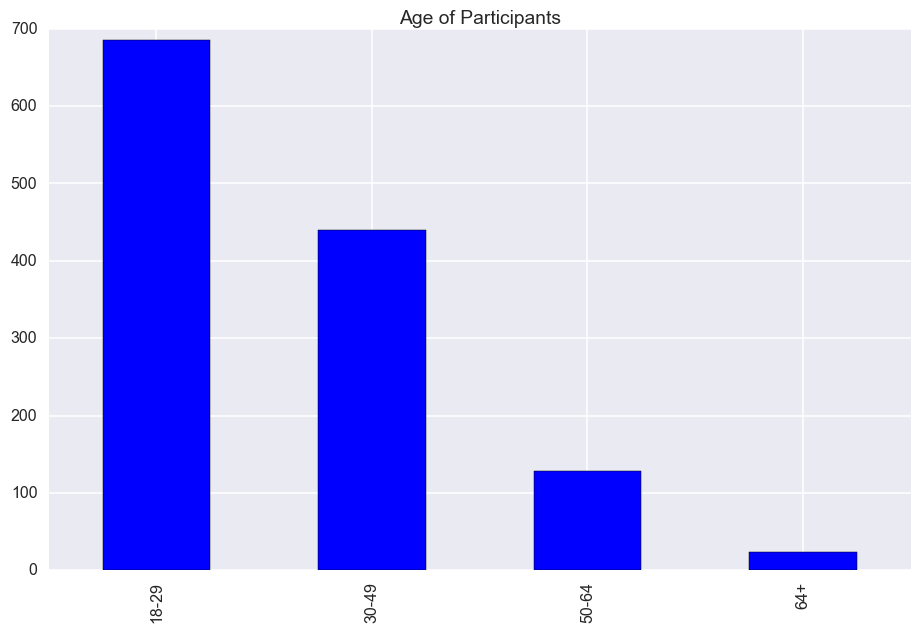
\includegraphics[width=0.49\textwidth]{age_study2} 
  %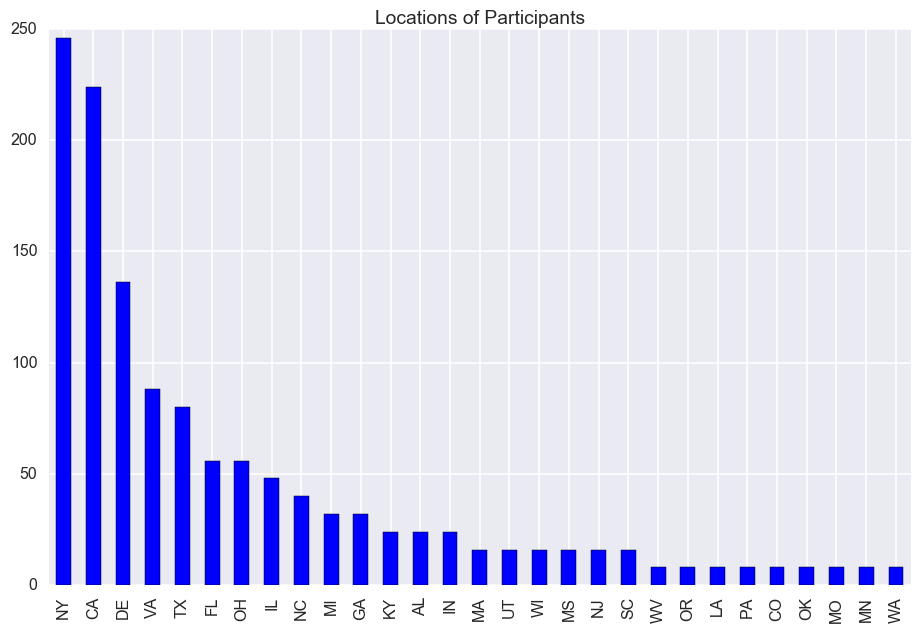
\includegraphics[width=0.32\textwidth]{location_study2} 
  \caption{Demographics of Participants
    \label{fig:demographics2}}
\end{figure}

Gender of participants were majority male. We had 758 male participants, 496 female participants and 24 signed up as ``other'' (it is possible that those who did not wish to identify chose the ``other'' category). 

Majority of participants were also in age group 18-29.
 
In our analyses, we balance for gender and age disparaties. %%%%% DO THIS !!!!!!!!!!!!!!!!!!!!!!

\subsection{Location}

Our participants represented a wide variety of geographic locations in the US.

\begin{figure}[H]  
\centering  
  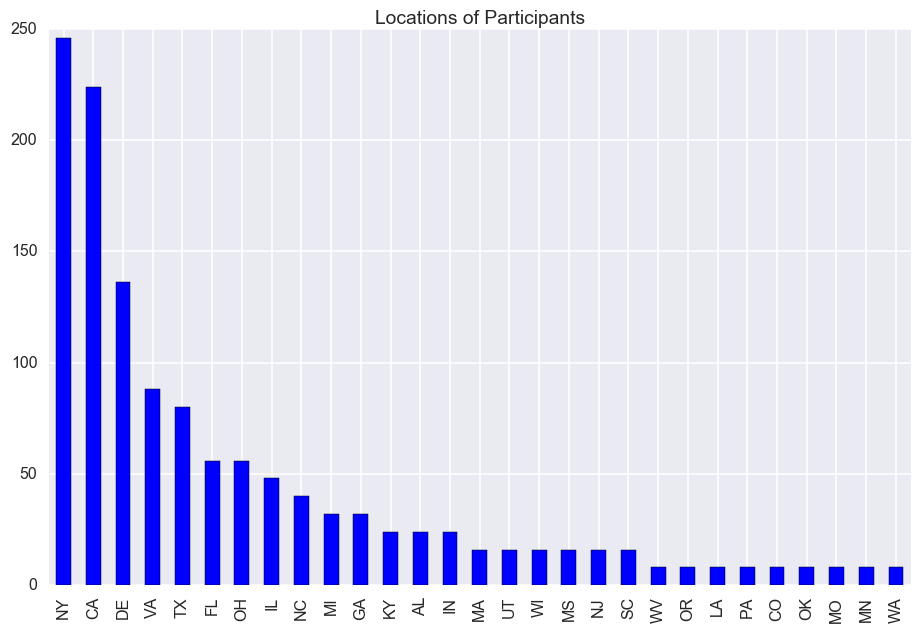
\includegraphics[width=0.9\textwidth]{location_study2} 
  \caption{Locations of Participants
    \label{fig:locations2}}
\end{figure}

\subsection{Political Affiliation}

More than twice as many democrats than republicans particpated in our study, which also was reflected in candidate preference disparaties. These effects are taken into account in our modeling.

\begin{figure}[H]  
\centering 
  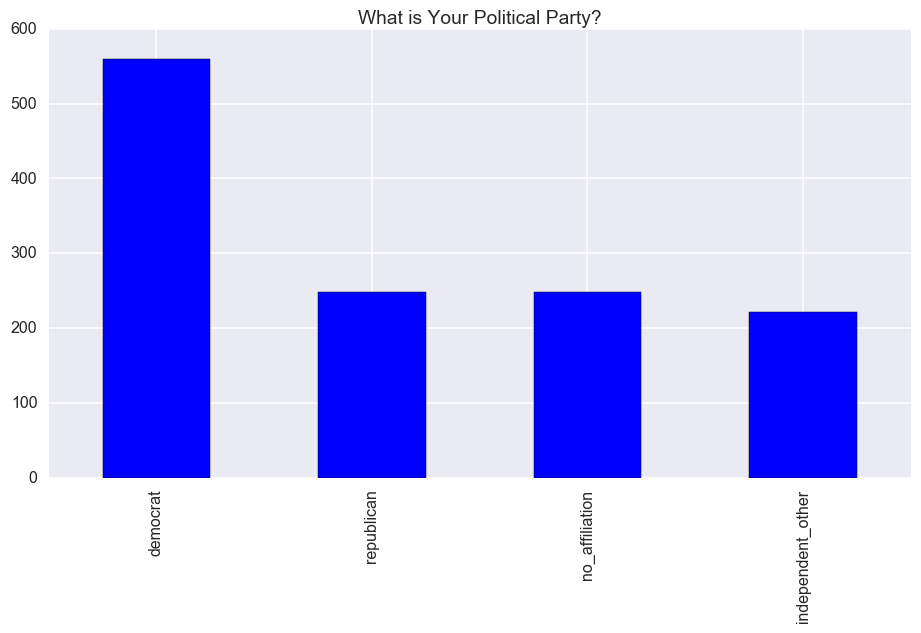
\includegraphics[width=.7\textwidth]{party_study2} 
  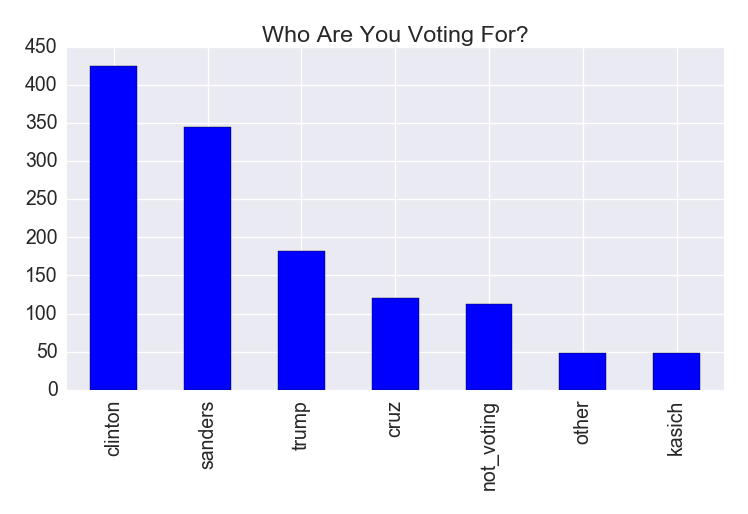
\includegraphics[width=.7\textwidth]{voting_for_study2}  
  \caption{Political Affiliations of Participants
    \label{fig:political2}}
\end{figure}

 
  
% See figure~\ref{fig:demographics2} on page \pageref{fig:demographics2}

% See figure~\ref{fig:locations2}
% See figure~\ref{fig:party2}

\newpage
\subsection{Trust}
From a scale of -2 (Strongly Disagree) to 2 (Strongly Agree), on average, most stories were deemed trustworthy for all groups with a mean score of 0.55 (between Neutral and Agree). For distribution of all scores, see figure~\ref{fig:trust} on page \pageref{fig:trust}.

However, the distrubtions for candidates varied. Stories about Sanders were seen as most trustworthy across all participants with a mean score of 0.66, followed by Cruz (0.63), Clinton (0.53), and Trump (0.40).

\begin{figure}[H] 
\centering 
  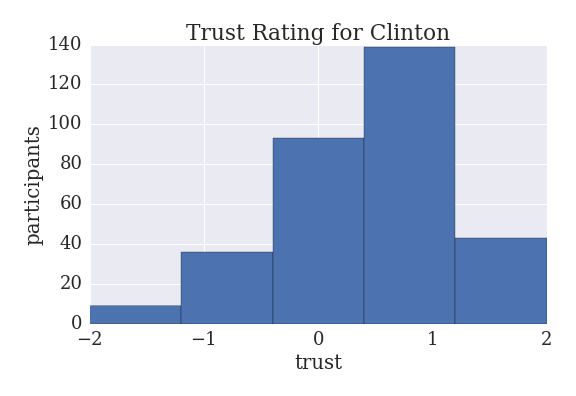
\includegraphics[width=.49\textwidth]{trust_clinton}   
  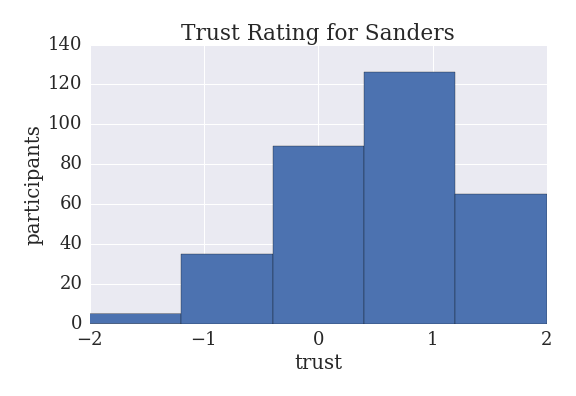
\includegraphics[width=.49\textwidth]{trust_sanders}   
  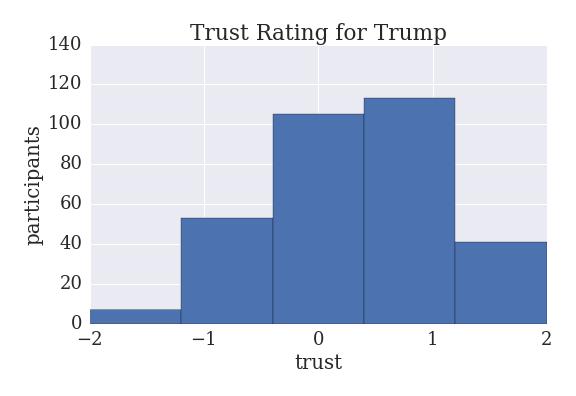
\includegraphics[width=.49\textwidth]{trust_trump}   
  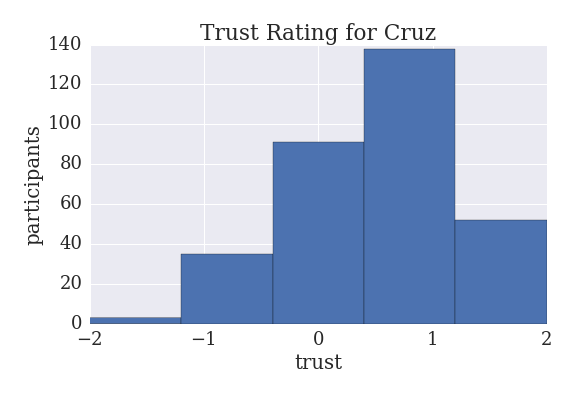
\includegraphics[width=.49\textwidth]{trust_cruz}  
  \caption{Trust Ratings for Stories About Candidate
    \label{fig:trust}}   
\end{figure}

On average, men were slightly less likely to trust stories (average of 0.54) than women (0.60) and others. 

Those in age group 30-49 were most likely to find stories trustworthy (average 0.675), followed by those in age group 50-64 (average 0.083), then those 18-29 (0.49), then those 64+ (0.083).

For distributions of trust by age group, see figure~\ref{fig:trust-by-age} on page \pageref{fig:trust-by-age}.

On average, stories were more trusted by democrats (0.69 mean).

% FIX THIS !!!!!!!!!!
For distributions of trust by party affiliation, see figure ?? on page ??.

\subsection{Fairness}
From a scale of -2 (Strongly Disagree) to 2 (Strongly Agree), on average, most stories were deemed fair for all groups with a mean score of 0.57 (between Neutral and Agree). For distribution of all scores, see figure~\ref{fig:fair} on page \pageref{fig:fair}.

Perceptions of fair treatment of candidates in stories diverged from the trust ratings above. Whereas stories about Sanders were most trusted, those about Clinton were seen as most fair (0.67 average).

\begin{figure}[H] 
\centering 
  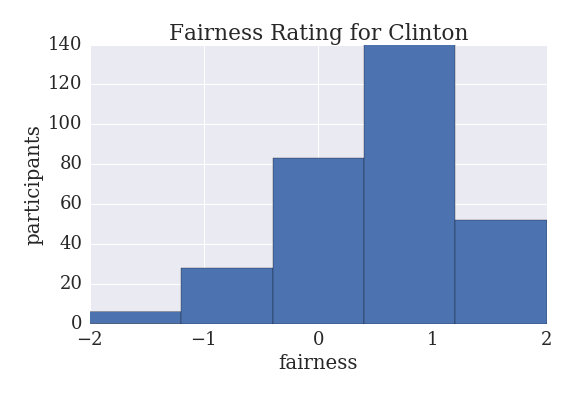
\includegraphics[width=.49\textwidth]{fair_clinton}   
  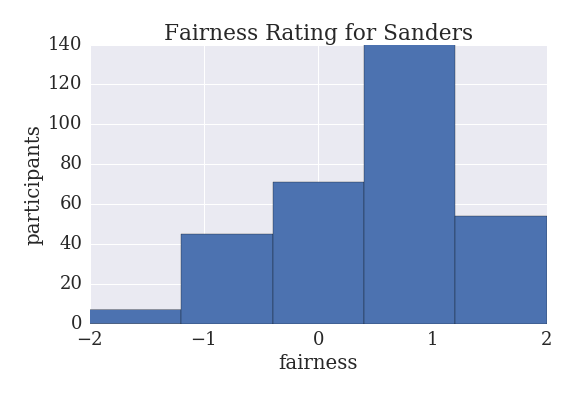
\includegraphics[width=.49\textwidth]{fair_sanders}   
  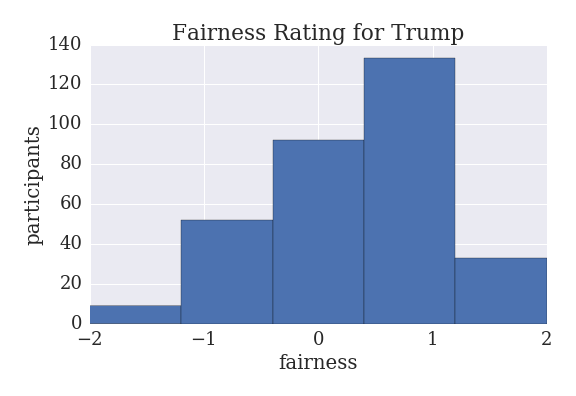
\includegraphics[width=.49\textwidth]{fair_trump}   
  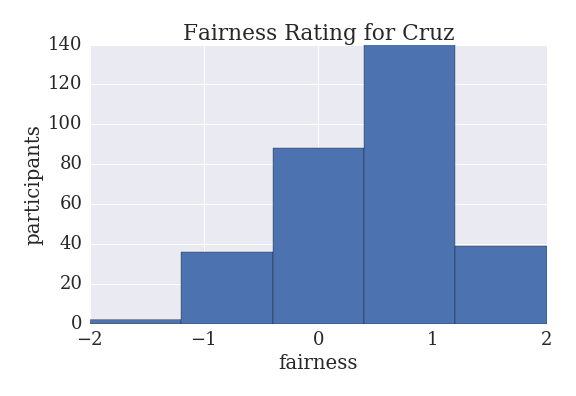
\includegraphics[width=.49\textwidth]{fair_cruz}  
  \caption{Fairness Ratings for Stories About Candidate
    \label{fig:fair-candidate}}   
\end{figure}

Women were more likely to see articles as fair on average (0.67) than men (0.51 mean).
Again, those in age group 30-49 were also most likely to find stories fair (average .70), this time followed by Millenials (0.51 average), then those 50-64 (0.48) and 64+ (0.20).

Democrats and Independents were far more likely to view stories as fair on average (0.68, 0.67) than Republicans (0.375), although all averages were between neutral and fair.

This finding about low perceptions of fairness in media is aligned with prior research findings. In ``The Liberal Media Myth Revisited,'' T.T. Lee hypothesized (and verified) that ``the more conservative (versus liberal) media consumers are, the more likely they are to perceive a media bias'' and similarly ``the more consumers lean toward the Republican (versus Democratic) party, the more likely they are to perceive a media bias'' \cite{lee2005liberal}.
% For distributions of trust by age group, see figure~\ref{fig:trust-by-age} on page \pageref{fig:trust-by-age}.

% On average, stories were more trusted by democrats (0.69 mean).

% % FIX THIS !!!!!!!!!!
% For distributions of trust by party affiliation, see figure ?? on page ??.
 

%% FUN SECTION: COMMENTS COLLECTED
 
\section{Reading Level Effects}


\section{Media Brand Effects}

\section{Qualitative}
People's comments
And whether or not they read the stories

\section{Conclusions}

How do your trustworthiness findings line up with the findings from Pew surveys and prior work? What hypotheses did you verify from prior work?

\section{Limitations}

Our study shows significant effects that open potential new areas of experimentation while confirming past theories of how media bias is formed. In the interest of focus, our study centered around four candidates and a narrowed dataset of eight stories, but in the future could be replicated on a larger set of more diverse stories and outlets. 

Furthermore, although the contributor market on CrowdFlower is not representative of any specific region or demographic, it is also not representative of the nation at large.

\part{Sharing the News}
\chapter{Exploratory Study}

\section{Motivation}
What was the purpose of the study?
What were the hypotheses?

\section{Dataset}
What was the dataset?


How did you get the dataset?
 

Why those sources?
 


% What’s CrowdFlower?
 
% What’s the difference between CrowdFlower and Turk?
 

% How did you control for quality?

% CrowdFlower has a built-in “Test Question” feature that allows for the rejection of a annotator whose answers to specific questions do not lie within a threshold (default 70%) of the “correct” answer or whose answers lay outside the standard variation compared to others.

% However, since the questions we asked were by nature subjective and therefore outliers and disagreements in answers could imply signal rather than noise, we chose to monitor for quality using other metrics instead. CrowdFlower was not designed explicitly for survey-like tasks, and therefore there were no options for different screening methods or questions. Gold Questions on the platform are selected by the creator within the set of all questions being recorded.

% Because of this, we monitored quality of results in two ways:

% First, by setting a minimum of time of 180 seconds to complete the task of reading 5 stories for a task to be accepted,

% And second, by selecting only Level 3 workers on CrowdFlower as suggested on their website for handling survey-like tasks.
% [https://success.crowdflower.com/hc/en-us/articles/201855969-Survey-Guide-To-Running-Surveys] 

% Users were also only allowed to answer the set of questions once. 

% Average response time was 07:31 minutes.
 

 
% What kind of people signed up for your study?

 
% What was the duration, n size, etc.
 

% How did you recruit them? What was their incentive?
 

% What kind of effects were you looking for?
 
% What kind of effects did you find?

% Trustworthiness

% How do your trustworthiness findings line up with the findings from Pew surveys?

% What about favorability?
  




  


% Basic stats here:
% we ran over X days
% over data points

% \section{Reader Demographics}

% \section{Media Favorability of Candidates}
% Each reader was asked to score the five stories according to how favorable each one was to the featured candidate (by headline). 

% \begin{figure}[h!] 
% \centering
%   \fbox{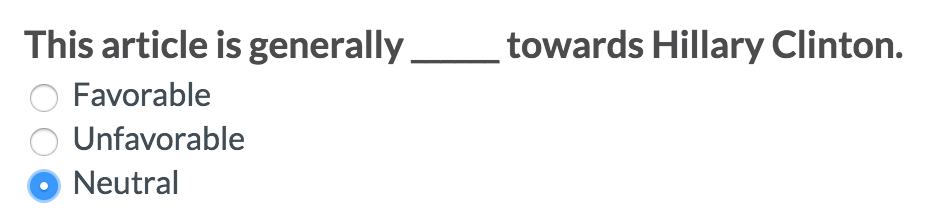
\includegraphics[width=0.5\textwidth]{favorability_question}}
%   \caption{Example of favorability scoring question}
% \end{figure}
 
% Scores were collected on a three-point scale, Favorable (1), Unfavorable (-1), or Neutral (0).

% Overall, media coverage of Trump was viewed as most negatively biased, with over half of stories (51.1\%) viewed as unfavorable towards the candidate.

% Of the stories shown, both Sanders and Clinton were viewed as having more positive than negative coverage, at 38.9\% of the 180 annotations being positive. Sanders also had the least negative coverage, with only 18.3\% stories shown being viewed as negatively biased against the candidate. Republican candidate Cruz was also seen to have more negative (33.3\%) than positive (28.9\%) stories about him, although the majority were seen as neutral (37.8\%).

% \begin{figure}[h!] 
% \centering
%   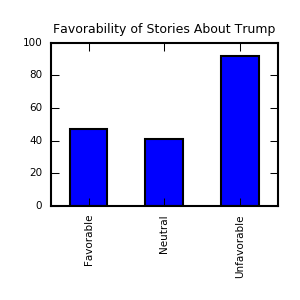
\includegraphics[width=0.45\textwidth]{Trump_favorability} 
%   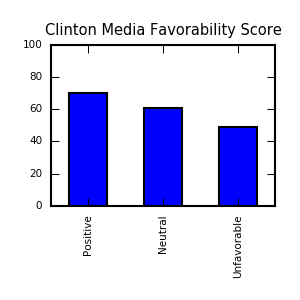
\includegraphics[width=0.45\textwidth]{Clinton_favorability} 
%   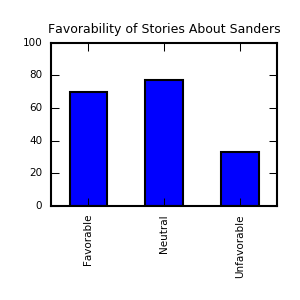
\includegraphics[width=0.45\textwidth]{Sanders_favorability} 
%   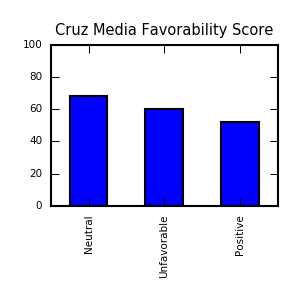
\includegraphics[width=0.45\textwidth]{Cruz_favorability} 
%   \caption{Media Favorability of Candidates}
% \end{figure}

% These trends persist when we filter responses by stories that were considered trustworthy or at least neutral (score > 0).

% \begin{figure}[h!] 
% \centering
%   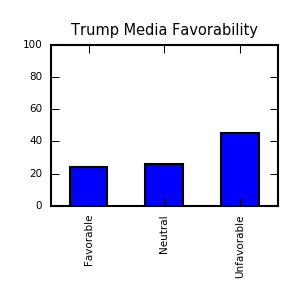
\includegraphics[width=0.45\textwidth]{Trump_favorability_trust_gt_0} 
%   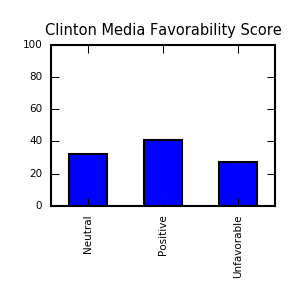
\includegraphics[width=0.45\textwidth]{Clinton_favorability_trust_gt_0} 
%   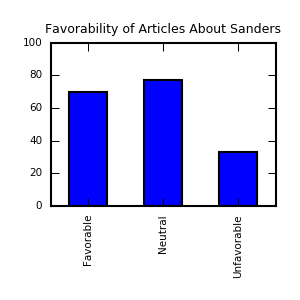
\includegraphics[width=0.45\textwidth]{Sanders_favorability_trust_gt_0} 
%   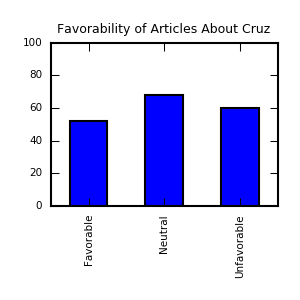
\includegraphics[width=0.45\textwidth]{Cruz_favorability_trust_gt_0} 
%   \caption{Media Favorability of Candidates, Trustworthy Articles}
% \end{figure}

% In the following section, we examine more patterns of media trustworthiness.


% \section{Media Trustworthiness}

% Each reader was also asked to score the five stories according to how trustworthy they found each to be. 

% \begin{figure}[h!] 
% \centering
%   \fbox{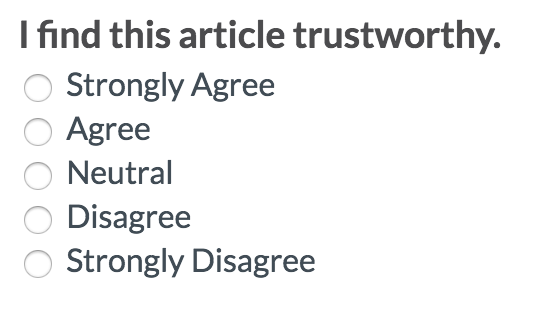
\includegraphics[width=0.35\textwidth]{trustworthy_question}}
%   \caption{Example of trustworthiness scoring question}
% \end{figure}

% Scores were collected on a five-point (Likert) scale: Strongly Agree (2), Agree (1), Neutral (0), Disagree (-1), Strongly Disagree (-2). Overall, readers seldom slected ``Strongly Disagree'', and the option consisted of less than 2\% of all choices.

% In the analysis below, we collapse the results into three categories: Agree (> 0), Neutral (0), and Disagree (<0).

% Despite reportings on national distrust of news, the majority of stories were marked as trustworthy for all candidates.

% \begin{figure}[h!] 
% \centering
%   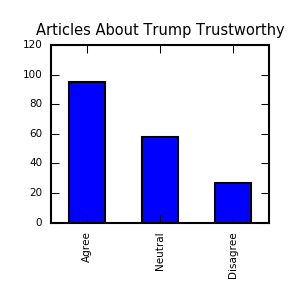
\includegraphics[width=0.45\textwidth]{Trump_trustworthiness_binary} 
%   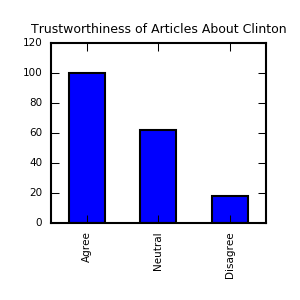
\includegraphics[width=0.45\textwidth]{Clinton_trustworthiness_binary} 
%   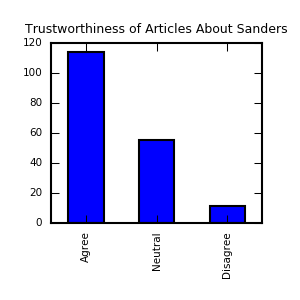
\includegraphics[width=0.45\textwidth]{Sanders_trustworthiness_binary} 
%   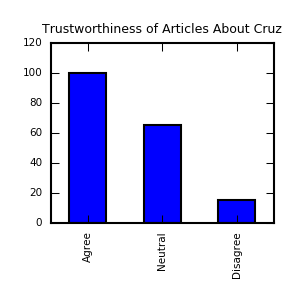
\includegraphics[width=0.45\textwidth]{Cruz_trustworthiness_binary} 
%   \caption{Media Trustworthiness of Candidate Coverage}
% \end{figure}

%  Sanders has strongest trustworthiness, most favorable



 

% \section{Overall Bias Reportings}


% \section{Media Brand Effect}

% \section{Reading Level Effect}

% \section{Other Linguistic Cues}

\section{Limitations}

From our exploratory study, we were able to obtain a significant but weak effect between disclosing the source and the levels of trust marked by readers towards an article.

We also observed trends that suggested an interaction between disclosing the source and the reading level of a story.

However, the study faced several limitations: first, we did not obtain enough samples to show a statistically significant result for interactions between source and reading level.

Furthermore, multiple levels of independent variables (ie: 5 levels for input source) made modeling complex and the results less clear.

The dataset was also unbalanced and sparse (ie, because of large numbers of input variables we did not have complete representation for each category, such as high, low, and mid-reading level stories for every outlet and topic). We tried to control for those factors by randomization, however it made more difficult to analyze specific correlations between source and trust.

To further explore the interaction between disclosing the source and the reading level of the story, we set up another crowdsourcing experiment on CrowdFlower, this time targeting this specific interaction, to see if there is a significant effect between the two, detailed in the following chapter.

% % This is an example of how you would use tgrind to include an example
% % of source code; it is commented out in this template since the code
% % example file does not exist.  To use it, you need to remove the '%' on the
% % beginning of the line, and insert your own information in the call.
% %
% %\tagrind[htbp]{code/pmn.s.tex}{Post Multiply Normalization}{opt:pmn}
%    
\chapter{Conclusion}
 \chapter{Metrics for Analysis}
\section{Independent Variables}
\section{Emotional Coding}


$$ emotionality = \frac{count(positiv \mid negativ)}{count(words)}$$
$$ positivity = \frac{count(positiv)}{count(words)} - \frac{count(negativ)}{count(words)}$$


 \section{Followership as a Proxy for Political Engagement}
In the following sections, we use Twitter followership as a proxy for measuring degrees of political engagement. 

Previous research in network analysis and attempts to predict latent political affiliations of users in the social network has shown that users on Twitter tend to show network homophily within political groups, and that ``like follows like'' \cite{colleoni2014echo}. In addition, followership of only Democratic or only Republican official accounts can be used as a reasonable estimator of party loyalty. Those accounts that follow only the officials of one party tend to demonstrate more closeness with other users in their political party than those who do not.
            
Due to the highly individual nature of this election, where candidate loyalty does not necessarily imply goodwill towards the party, we look specifically at what candidates users follow instead of party loyalty at large. 

For \emph{levels} of political engagement, we group those Twitter users who share news stories into three segments: 

\begin{itemize}
  \item \emph{the unaffiliated} (those who follow no presidential candidates, but do tweet about political news)
  \item \emph{single-candidate} Tweeters (those who follow one and only one presidential candidate, and tweet about political news)
  \item \emph{political aficionados} (those who follow all 4 (or more) candidates, and tweet about political news)
\end{itemize}

In addition, for single-candidate Tweeters, we divide users by the candidate they follow. At the time of data collection completion (May 1, 2016), the top two candidates by delegate count in each party were Hillary Clinton (D), Bernie Sanders (D) and Donald Trump (R) and Ted Cruz (R), so we split users into these four groups. We call each group \emph{X}-followers where \emph{X} is the candidate name, although these do not include every person on Twitter who follows \emph{X}.  
%  \chapter{The Electome Project}
%  % intro-y to electome here
%  % cite its outcomes 
 

% \section{Motivation}
% \section{Approach}
% \section{Applications}
\chapter{Conclusion}
 \chapter{Metrics for Political and Emotional Engagement}

 In the following sections, we discuss the tools and methods that we use to analyze our independent variables.
 
\section{Emotional Coding}
For the emotional coding of news articles, we use dictionaries from the Harvard General Inquirer, a lexicon that is popular for computerized content analysis \cite{ stone1963computer}. The Inquirer is a public-use alternative to the LIWC system, which in Berger and Milkman’s study of online virality showed results that were significantly positively correlated with the output of manual coding \cite{berger2012makes}. In particular, we use the \emph{Positiv} and \emph{Negativ} collections, a set of 1,915 well-established words signifying positive outlook (not including words for \emph{yes}) and 2,291 words signifying negative outlook (not including words for \emph{no}), respectively. Repeating the same metrics from \emph{What Makes Online Content Viral?}, we quantify for each document:

$$ emotionality = \frac{count(positiv \mid negativ)}{count(words)}$$
$$ positivity = \frac{count(positiv)}{count(words)} - \frac{count(negativ)}{count(words)}$$

as independent variables in our analysis.

 \section{Followership as a Proxy for Political Engagement}

In the following sections, we use Twitter followership as a proxy for measuring degrees of political engagement. 

Previous research in network analysis and attempts to predict latent political affiliations of users in the social network has shown that users on Twitter tend to show network homophily within political groups, and that ``like follows like'' \cite{colleoni2014echo}. In addition, followership of only Democratic or only Republican official accounts can be used as a reasonable estimator of party loyalty. Those accounts that follow only the officials of one party tend to demonstrate more closeness with other users in their political party than those who do not.
            
Due to the highly individual nature of this election, where candidate loyalty does not necessarily imply goodwill towards the party, we look specifically at what candidates users follow instead of party loyalty at large. 

For \emph{levels} of political engagement, we group those Twitter users who share news stories into three segments: 

\begin{itemize}
  \item \emph{the unaffiliated} (those who follow no presidential candidates, but do tweet about political news)
  \item \emph{single-candidate} Tweeters (those who follow one and only one presidential candidate, and tweet about political news)
  \item \emph{political aficionados} (those who follow all 4 (or more) candidates, and tweet about political news)
\end{itemize}

In addition, for single-candidate Tweeters, we divide users by the candidate they follow. At the time of data collection completion (May 1, 2016), the top two candidates by delegate count in each party were Hillary Clinton (D), Bernie Sanders (D) and Donald Trump (R) and Ted Cruz (R), so we split users into these four groups. 

%We call each group \emph{X}-followers where \emph{X} is the candidate name, although these do not include every person on Twitter who follows \emph{X}.  

\subsection{A Look at Candidate Followership}

Our dataset contains 6,406 unique single-candidate Twitter users. Trump-only followers lead with about 31\%, followed closely by Clinton-only (29\%), then Sanders (25\%) and Cruz (14\%).

\begin{figure}[H] 
\centering 
 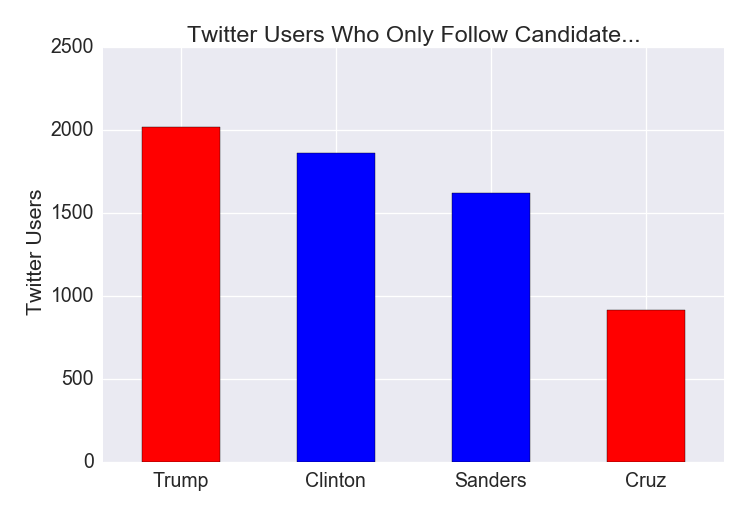
\includegraphics[width=0.8\textwidth]{users-by-candid}   
  %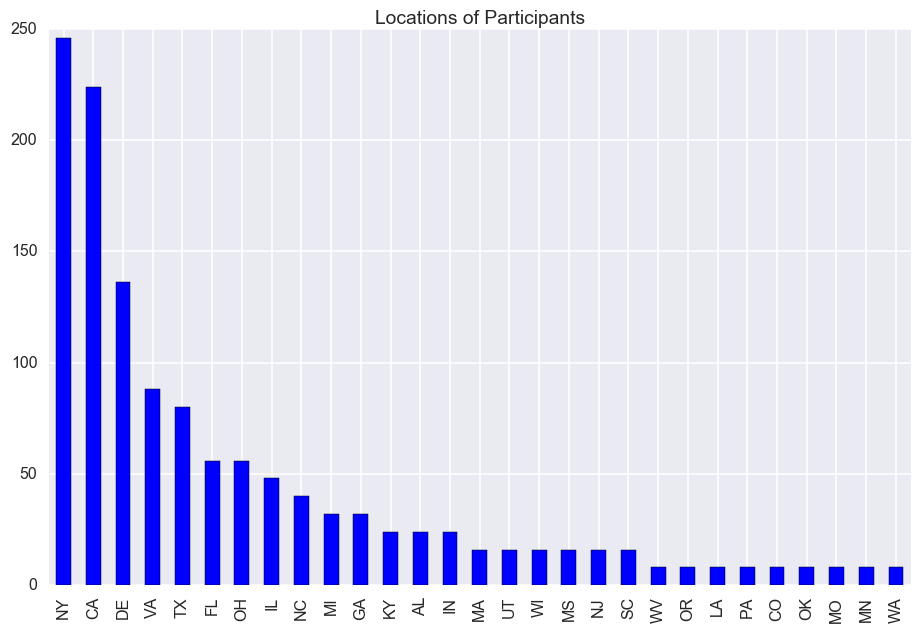
\includegraphics[width=0.32\textwidth]{location_study2} 
  \caption{User and Tweet Counts by Followership
    \label{fig:weets-by-candid}}
\end{figure}

Trump's free media advantage becomes clear when looking at the \emph{volume} of tweets each group of users tweet: 37\% of tweets sharing articles come from Trump-only followers versus 27\% for Clinton-only, 20\% for Sanders-only, and 14.6\% for Cruz.

\begin{figure}[H] 
\centering 
 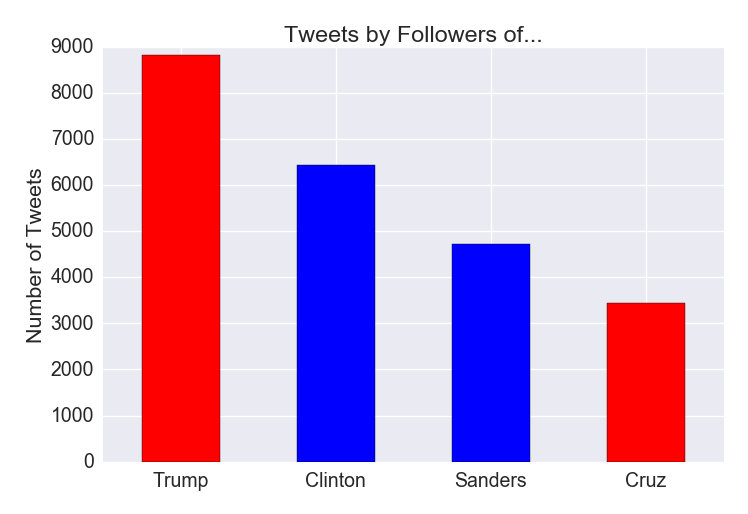
\includegraphics[width=0.8

 \textwidth]{tweets-by-candid}  
  %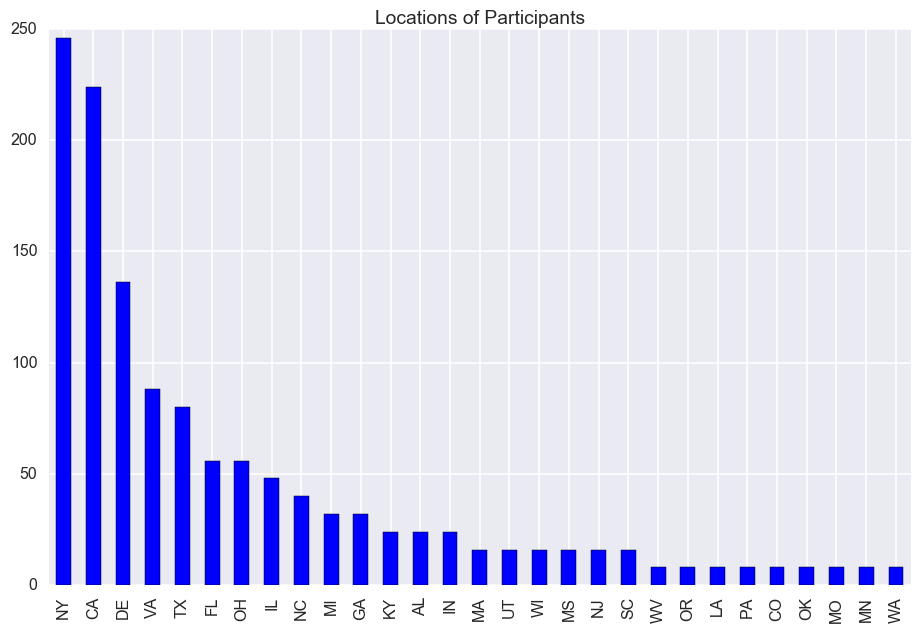
\includegraphics[width=0.32\textwidth]{location_study2} 
  \caption{User and Tweet Counts by Followership
    \label{fig:users-by-candid}}
\end{figure}


Although candidate-followership is only a proxy for the latent variable of candidate loyalty, we are observe the nature of the content being shared by each group. Again, across all four segments, Republican candidate Trump leads the top number of mentions in stories shared.

%% Most popular mentioned candidate by ea. camp
\begin{figure}[H] 
\centering 
 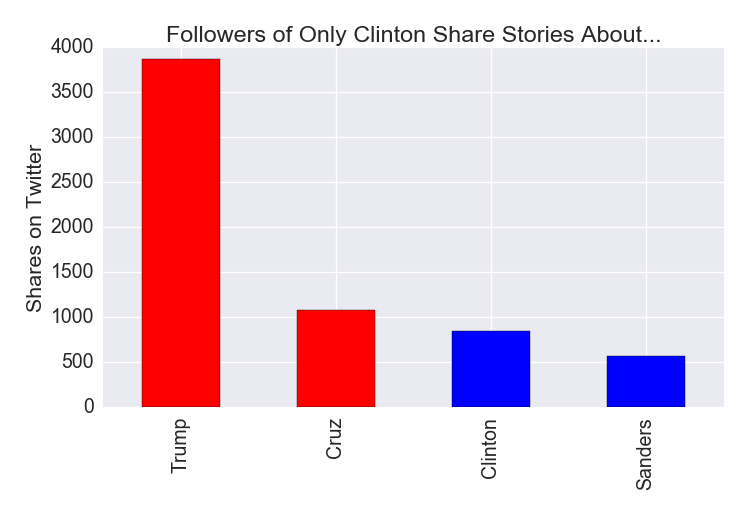
\includegraphics[width=0.49\textwidth]{clinton-camp-shares}
 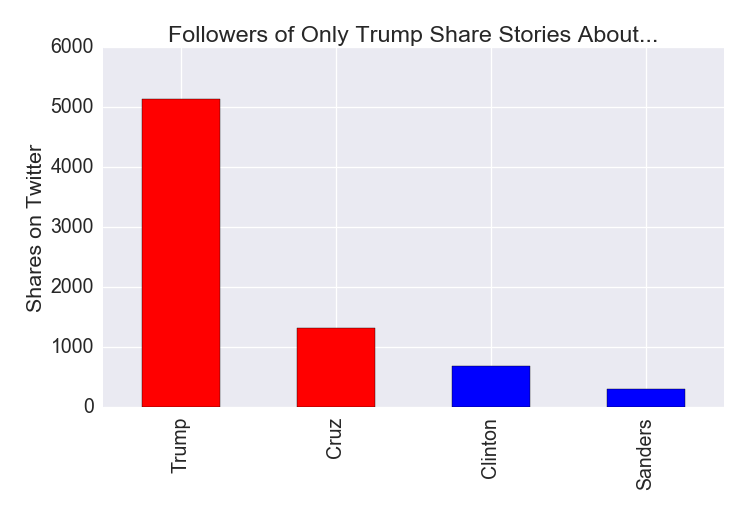
\includegraphics[width=0.49\textwidth]{trump-camp-shares}  
 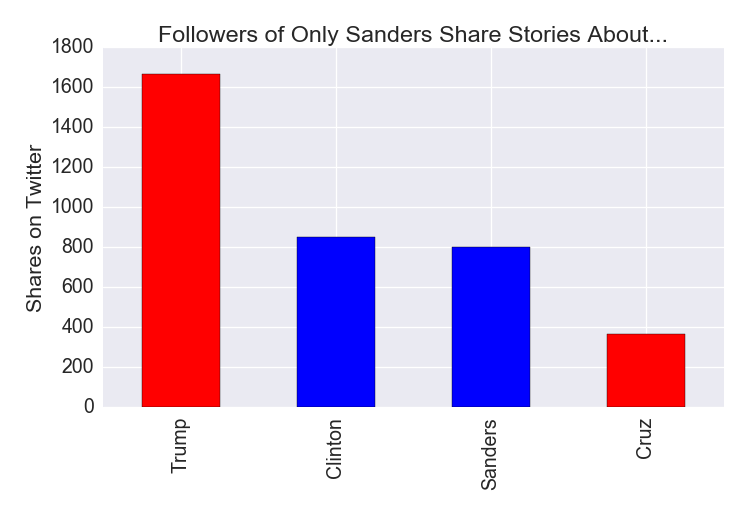
\includegraphics[width=0.49\textwidth]{sanders-camp-shares}  
 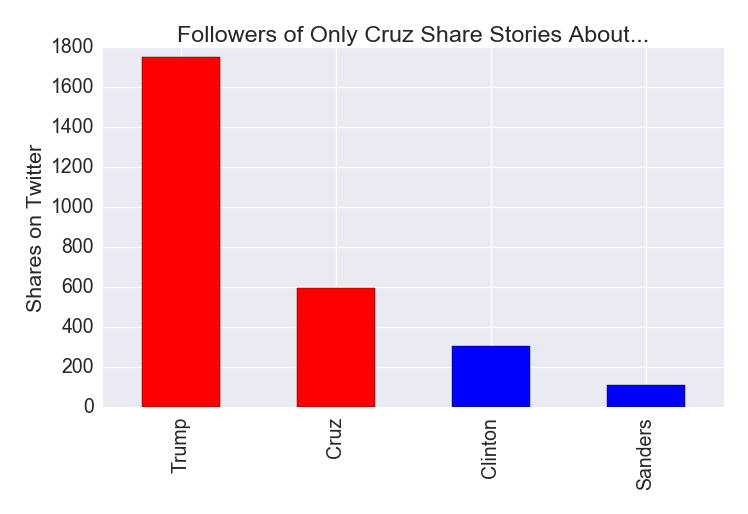
\includegraphics[width=0.49\textwidth]{cruz-camp-shares}  
  %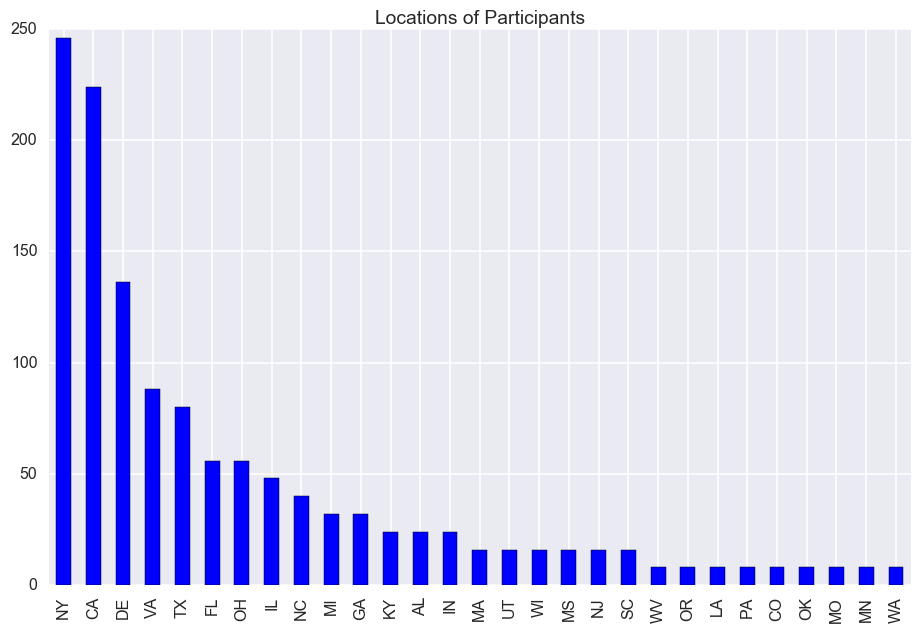
\includegraphics[width=0.32\textwidth]{location_study2} 
  \caption{Tweet and User Counts by Followership
    \label{fig:users-tweets-by-candid}}
\end{figure}
 
\subsection{A Look at Levels of Political Engagement}
Descriptives of candididate 0/1/3+:
* Bar chart of \% by \# Following
* Number of tweets by each camp
* Most popular orgs by each camp
* Most popular story by each camp
* Most mentioned candid in each camp










% * Top 10 by each camp

% %%% Trump

% \begin{table}
% \begin{tabular}{ |l c| } 
%     %s\toprule
%     \hline
%     Article &  \# tweets \\
%     \hline 
%     Donald Trump Is Shocking, Vulgar and Right                            &    221 \\
%     Trump basks in his spotlight                                          &     84 \\
%     Poll: Trump dominates GOP field                                       &     79 \\
%     The One Weird Trait That Predicts Whether You’re a Trump Supporter    &     75 \\
%     Why I'm voting for Trump                                              &     74 \\
%     Rubio: Law-abiding undocumented immigrants could stay                 &     73 \\
%     Poll: Donald Trump gained 15 points on Ted Cruz in Iowa in two weeks  &     69 \\
%     FOX NEWS POLL  Trump gains in Iowa, dominates New Hampshire           &     57 \\
%     TODD STARNES School caught trying to get students to work for Hillary &     57 \\
%     Poll: Evangelicals flocking to Trump                                  &     54 \\
%      \hline
% \end{tabular}
% \caption{\label{tab:top-10}Top 10 Shared By Trump Followers}
% \end{table}

% %%% Clinton
% \begin{table}
% \begin{tabular}{ |l c| } 
%     %s\toprule
%     \hline
%     Article &  \# tweets \\
%     \hline 
%     The One Weird Trait That Predicts Whether You’re a Trump Supporter                            &    115 \\
%     I Get Sanders’ Appeal. But He’s Not a Credible President.                                     &     74 \\
%     Ted Cruz Is No Jack Kennedy                                                                   &     68 \\
%     Why I'm voting for Trump                                                                      &     50 \\
%     Anne Frank's stepsister compares Donald Trump to Adolf Hitler                                 &     46 \\
%     Poll: Clinton has a better shot at beating Trump than Sanders                                 &     42 \\
%     Judge dismisses lawsuits over Clinton's emails                                                &     34 \\
%     Terrorists use Trump's `Muslim ban' speech in recruitment video                               &     33 \\
%     Trump’s Campaign Is Damaging His Brand                                                        &     27 \\
%     Donald Trump is not beating Hillary Clinton in the polls, no matter how many times he says it &     27 \\
%      \hline
% \end{tabular}
% \caption{\label{tab:top-10-clinton}Top 10 Shared By Clinton Followers}
% \end{table}


% %%% Sanders
% \begin{table}
% \begin{tabular}{ |l c| } 
%     %s\toprule
%     \hline
%     Article &  \# tweets \\
%     \hline 
%     The One Weird Trait That Predicts Whether You’re a Trump Supporter                  &    136 \\
%     Bernie Sanders Will Win Iowa, New Hampshire, Nevada and South Carolina. Here's Why. &    104 \\
%     Bernie Sanders Is a Once in a Lifetime Presidential Candidate. The Time Is Now.     &     99 \\
%     On January 20, 2017 Bernie Sanders Will Be Sworn In as America's 45th President     &     98 \\
%     Biden praises Sanders on income inequality                                          &     91 \\
%     Hillary's Corporate Democrats Taking Down Bernie Sanders                            &     91 \\
%     Bernie Sanders Is Now the `Inevitable' Democratic Nominee and Presidential Winner   &     90 \\
%     How the media missed Sanders                                                        &     83 \\
%     The Nation endorses Bernie Sanders                                                  &     74 \\
%     State Department asks for deadline extension on Hillary Clinton emails              &     72 \\
%     \hline
% \end{tabular}
% \caption{\label{tab:top-10-sanders}Top 10 Shared By Sanders Followers}
% \end{table}


% %%% Cruz
% \begin{table}
% \begin{tabular}{ |l c| } 
%     %s\toprule
%     \hline
%     Article &  \# tweets \\
%     \hline 
% Donald Trump attacks evangelical leader in Iowa who endorsed Ted Cruz                  &     60 \\
% Rubio: Law-abiding undocumented immigrants could stay                                  &     57 \\
% Donald Trump Is Shocking, Vulgar and Right                                             &     43 \\
% Let's uproot the pernicious, unproven claim that Ted Cruz attacked Donald Trump's wife &     43 \\
% TODD STARNES School caught trying to get students to work for Hillary                  &     43 \\
% The One Weird Trait That Predicts Whether You’re a Trump Supporter                     &     32 \\
% How the RNC squashed its only conservative-media debate                                &     21 \\
% NEXT ROUND: Fox News announces lineup for GOP prime time debate                        &     20 \\
% BATTLE FOR THE GOP RNC cuts debate ties with mag over anti-Trump issue                 &     18 \\
% BLOOMING CANDIDACY? Former NYC mayor reportedly mulling WH bid                         &     18 \\
%     \hline
% \end{tabular}
% \caption{\label{tab:top-10-sanders}Top 10 Shared By Sanders Followers}
% \end{table}

 
% \subsection{Who Are Single-Candidate Tweeters?}
% A qualitative peek into the characteristics of single-candidate tweeters shows a reasonable proxy for candidate loyalty. Examining the top 10 followers for each candidate by volume of tweets shared by each in our dataset, we see a mix of personal, organizational, and other accounts.

% Below is a random sample of the profile descriptions of 10 single-candidate tweeters (usernames excluded for the sake of privacy):
 
% \begin{itemize}  

% \item\emph{Clinton follower}: I write about climate change, Nikola Tesla, and Abraham Lincoln. Oh, and I'm an aquarium nut. Go figure.

% \item\emph{Trump follower}: Trump supporter, free-lance writer, loves life, liberty \& the pursuit of happiness

% \item \emph{Sanders follower}: I am an Android. MUST NOT SLEEP; MUST WARN OTHERS

% \item \emph{Clinton follower}: Love a little political humor? Then Letters From Us is the site for you. Check us out for new daily blogs and comics to feed your left-brain.

% \item \emph{Trump follower}: I am a former Marine (E-5 Sergeant.)I am a proponent of eradicating a welfare state.  I am appalled by the degradation of society by the liberal establishment
 
% \item \emph{Trump follower}: We bring you the biggest breaking stories all over the world. We have online journalists that are experienced \& caffeinated. with @JoshiiHD \& DaviiHD
 
% \item \emph{Clinton follower}: Media Critic/Journalist/Hillary 4 Am. Vol. Leader ~Prolific!!! Bad Manners Blocked! Blogs: https://t.co/KraI7CJNlD \& https://t.co/WRcDx0bP63 \#PDMFNB \#UniteBlue
 
% \item \emph{Sanders follower}: I am not accepting new clients. I am on vacation and not eligible to practice law until July 15, 2016.

% \item \emph{Clinton follower}: Graduate of Delaware State, U of Penn, Bowie Md and Temple U

% \item \emph{Cruz follower}: Conservative, Christian, Farm wife to @1861\_again, Stay at home mom of 3 boys, Gardner, Altrium health suppliment dealer, Strict Constitutionalist, Former Nurse

% \end{itemize}

  
\chapter{Conclusion}

\section{Findings}

\section{Potential Impact}

\section{Limitations}
We found these effects, so what?
 
\subsection{Data Collection}
* obviously sources are a small set, might not be representative
* matching tweets and stories this way using regex is fast but might not be complete

 

%%% this is part I conlcusion ! move up!
% Media distrust, which has intensified over the last two decades, is a phenomenon with serious implications in the practice of democracy and a well-informed public.  

% In an election year prefaced by deep cynicism towards American institutions (a 2015 survey showed that just 19\% of the population trusts the federal government), attitudes towards the news media fare no better. Almost two-thirds of Americans think that the national news media is a negative influence on the country \cite{beyond-distrust}. 

% Our results confirm previous hypotheses about the importance of the role of the reader in determining news trust and bias \emph{over} the role of the content itself. We show that drastically different use of language complexity has little effect on the reader in comparison to the presence of media brands.

% Interestingly, although showing media from outlets of opposing political orientations decreases trust and fairness perceptions in the reader, when no outlet is attributed to the story, trust in the story also decreases. This suggests that interventions designed to \emph{level} news stories by aggregating them without attribution to source might not be effective in creating a balanced news diet for sustaining informed voters. 
\appendix
\chapter{Tables}
 %%%%%%%%%%%%%%%%%%%%% The unaffiliated %%%%%%%%%%%%%%%%%%%%%%%%%%%%%%%%%
\begin{table}[!htbp] \centering 
  \caption{Tweet Volume vs. Story Length, the Unaffiliated} 
  \label{} 
    \begin{tabular}{@{\extracolsep{5pt}}lccc} 
    \\[-1.8ex]\hline 
    \hline \\[-1.8ex] 
     & \multicolumn{3}{c}{\textit{Dependent variable:}} \\ 
    \cline{2-4} 
    \\[-1.8ex] & \multicolumn{3}{c}{Number of Tweets} \\ 
    \\[-1.8ex] & \textit{OLS} & \textit{Poisson} & \textit{negative} \\ 
     & \textit{} & \textit{} & \textit{binomial} \\ 
    \\[-1.8ex] & (1) & (2) & (3)\\ 
    \hline \\[-1.8ex] 
     Story length & $-$0.008$^{***}$ & $-$0.0004$^{***}$ & $-$0.0003$^{***}$ \\ 
      & (0.001) & (0.00001) & (0.00002) \\ 
      & & & \\ 
     Constant & 35.299$^{***}$ & 3.683$^{***}$ & 3.605$^{***}$ \\ 
      & (1.168) & (0.006) & (0.031) \\ 
      & & & \\ 
    \hline \\[-1.8ex] 
    Observations$^{*}$ & 2,640 & 2,640 & 2,640 \\ 
    R$^{2}$ & 0.029 &  &  \\ 
    Adjusted R$^{2}$ & 0.028 &  &  \\ 
    Log Likelihood &  & $-$49,432.820 & $-$11,415.510 \\ 
    $\theta$ &  &  & 0.954$^{***}$  (0.024) \\ 
    Akaike Inf. Crit. &  & 98,869.640 & 22,835.020 \\ 
    Residual Std. Error & 38.604 (df = 2638) &  &  \\ 
    F Statistic & 77.414$^{***}$ (df = 1; 2638) &  &  \\ 
    \hline 
    \hline \\[-1.8ex] 
    \textit{Note:}  & \multicolumn{3}{r}{$^{*}$p$<$0.1; $^{**}$p$<$0.05; $^{***}$p$<$0.01;} \\  
    \end{tabular}   
\end{table} 
\emph{$^{*}$We exclude stories not shared by this segment.}  
\newpage 
% Table created by stargazer v.5.2 by Marek Hlavac, Harvard University. E-mail: hlavac at fas.harvard.edu
% Date and time: Sun, Jul 24, 2016 - 19:08:45
\begin{table}[!htbp] \centering 
  \caption{Tweet Volume vs. Emotionality, the Unaffiliated} 
      \label{} 
    \begin{tabular}{@{\extracolsep{5pt}}lccc} 
    \\[-1.8ex]\hline 
    \hline \\[-1.8ex] 
     & \multicolumn{3}{c}{\textit{Dependent variable:}} \\ 
    \cline{2-4} 
    \\[-1.8ex] & \multicolumn{3}{c}{Number of Tweets} \\ 
    \\[-1.8ex] & \textit{OLS} & \textit{Poisson} & \textit{negative} \\ 
     & \textit{} & \textit{} & \textit{binomial} \\ 
    \\[-1.8ex] & (1) & (2) & (3)\\ 
    \hline \\[-1.8ex] 
     Emotionality & 248.768$^{***}$ & 8.165$^{***}$ & 7.427$^{***}$ \\ 
      & (79.579) & (0.347) & (2.145) \\ 
      & & & \\ 
     Constant & 22.519$^{***}$ & 3.147$^{***}$ & 3.162$^{***}$ \\ 
      & (1.747) & (0.008) & (0.047) \\ 
      & & & \\ 
    \hline \\[-1.8ex] 
    Observations$^{*}$ & 2,640 & 2,640 & 2,640 \\ 
    R$^{2}$ & 0.004 &  &  \\ 
    Adjusted R$^{2}$ & 0.003 &  &  \\ 
    Log Likelihood &  & $-$51,967.750 & $-$11,419.630 \\ 
    $\theta$ &  &  & 0.928$^{***}$  (0.023) \\ 
    Akaike Inf. Crit. &  & 103,939.500 & 22,843.260 \\ 
    Residual Std. Error & 39.094 (df = 2638) &  &  \\ 
    F Statistic & 9.772$^{***}$ (df = 1; 2638) &  &  \\ 
    \hline 
    \hline \\[-1.8ex] 
    \textit{Note:}  & \multicolumn{3}{r}{$^{*}$p$<$0.1; $^{**}$p$<$0.05; $^{***}$p$<$0.01} \\ 
    \end{tabular} 
\end{table}
\emph{$^{*}$We exclude stories not shared by this segment.}  
\newpage 
% Table created by stargazer v.5.2 by Marek Hlavac, Harvard University. E-mail: hlavac at fas.harvard.edu
% Date and time: Sun, Jul 24, 2016 - 19:09:28
\begin{table}[!htbp] \centering 
  \caption{Tweet Volume vs. Positivity, the Unaffiliated} 
  \label{} 
    \begin{tabular}{@{\extracolsep{5pt}}lccc} 
    \\[-1.8ex]\hline 
    \hline \\[-1.8ex] 
     & \multicolumn{3}{c}{\textit{Dependent variable:}} \\ 
    \cline{2-4} 
    \\[-1.8ex] & \multicolumn{3}{c}{Number of Tweets} \\ 
    \\[-1.8ex] & \textit{OLS} & \textit{Poisson} & \textit{negative} \\ 
     & \textit{} & \textit{} & \textit{binomial} \\ 
    \\[-1.8ex] & (1) & (2) & (3)\\ 
    \hline \\[-1.8ex] 
     Positivity & $-$145.324 & $-$5.277$^{***}$ & $-$4.036$^{*}$ \\ 
      & (90.790) & (0.440) & (2.452) \\ 
      & & & \\ 
     Constant & 27.797$^{***}$ & 3.324$^{***}$ & 3.321$^{***}$ \\ 
      & (0.795) & (0.004) & (0.021) \\ 
      & & & \\ 
    \hline \\[-1.8ex] 
    Observations$^{*}$ & 2,640 & 2,640 & 2,640 \\ 
    R$^{2}$ & 0.001 &  &  \\ 
    Adjusted R$^{2}$ & 0.001 &  &  \\ 
    Log Likelihood &  & $-$52,150.640 & $-$11,424.900 \\ 
    $\theta$ &  &  & 0.925$^{***}$  (0.023) \\ 
    Akaike Inf. Crit. &  & 104,305.300 & 22,853.790 \\ 
    Residual Std. Error & 39.147 (df = 2638) &  &  \\ 
    F Statistic & 2.562 (df = 1; 2638) &  &  \\ 
    \hline 
    \hline \\[-1.8ex] 
    \textit{Note:}  & \multicolumn{3}{r}{$^{*}$p$<$0.1; $^{**}$p$<$0.05; $^{***}$p$<$0.01} \\ 
    \end{tabular} 
\end{table}
\emph{$^{*}$We exclude stories not shared by this segment.} 
\newpage 

 %%%%%%%%%%%%%%%%%%% Single Candid %%%%%%%%%%%%%%%%%%%%%%%%%%%%%%%%%
% Table created by stargazer v.5.2 by Marek Hlavac, Harvard University. E-mail: hlavac at fas.harvard.edu
% Date and time: Sun, Jul 24, 2016 - 19:18:20
\begin{table}[!htbp] \centering 
  \caption{Tweet Volume vs. Story Length, Single-Candidate Followers} 
  \label{} 
    \begin{tabular}{@{\extracolsep{5pt}}lccc} 
    \\[-1.8ex]\hline 
    \hline \\[-1.8ex] 
     & \multicolumn{3}{c}{\textit{Dependent variable:}} \\ 
    \cline{2-4} 
    \\[-1.8ex] & \multicolumn{3}{c}{Number of Tweets} \\ 
    \\[-1.8ex] & \textit{OLS} & \textit{Poisson} & \textit{negative} \\ 
     & \textit{} & \textit{} & \textit{binomial} \\ 
    \\[-1.8ex] & (1) & (2) & (3)\\ 
    \hline \\[-1.8ex] 
     Story length & 0.002$^{***}$ & 0.0001$^{***}$ & 0.0002$^{***}$ \\ 
      & (0.0004) & (0.00001) & (0.00002) \\ 
      & & & \\ 
     Constant & 7.979$^{***}$ & 2.135$^{***}$ & 2.080$^{***}$ \\ 
      & (0.467) & (0.009) & (0.028) \\ 
      & & & \\ 
    \hline \\[-1.8ex] 
    Observations$^{*}$ & 2,581 & 2,581 & 2,581 \\ 
    R$^{2}$ & 0.007 &  &  \\ 
    Adjusted R$^{2}$ & 0.006 &  &  \\ 
    Log Likelihood &  & $-$17,969.510 & $-$8,449.973 \\ 
    $\theta$ &  &  & 1.330$^{***}$  (0.039) \\ 
    Akaike Inf. Crit. &  & 35,943.020 & 16,903.950 \\ 
    Residual Std. Error & 15.242 (df = 2579) &  &  \\ 
    F Statistic & 17.223$^{***}$ (df = 1; 2579) &  &  \\ 
    \hline 
    \hline \\[-1.8ex] 
    \textit{Note:}  & \multicolumn{3}{r}{$^{*}$p$<$0.1; $^{**}$p$<$0.05; $^{***}$p$<$0.01} \\ 
    \end{tabular} 
\end{table}
\emph{$^{*}$We exclude stories not shared by this segment.} 
\newpage 
% Table created by stargazer v.5.2 by Marek Hlavac, Harvard University. E-mail: hlavac at fas.harvard.edu
% Date and time: Sun, Jul 24, 2016 - 19:18:51
\begin{table}[!htbp] \centering 
  \caption{Tweet Volume vs. Emotionality, Single-Candidate Followers} 
  \label{} 
    \begin{tabular}{@{\extracolsep{5pt}}lccc} 
    \\[-1.8ex]\hline 
    \hline \\[-1.8ex] 
     & \multicolumn{3}{c}{\textit{Dependent variable:}} \\ 
    \cline{2-4} 
    \\[-1.8ex] & \multicolumn{3}{c}{Number of Tweets} \\ 
    \\[-1.8ex] & \textit{OLS} & \textit{Poisson} & \textit{negative} \\ 
     & \textit{} & \textit{} & \textit{binomial} \\ 
    \\[-1.8ex] & (1) & (2) & (3)\\ 
    \hline \\[-1.8ex] 
     Emotionality & 41.896 & 4.211$^{***}$ & 4.821$^{**}$ \\ 
      & (31.596) & (0.638) & (1.917) \\ 
      & & & \\ 
     Constant & 8.640$^{***}$ & 2.164$^{***}$ & 2.152$^{***}$ \\ 
      & (0.691) & (0.014) & (0.042) \\ 
      & & & \\ 
    \hline \\[-1.8ex] 
    Observations$^{*}$ & 2,581 & 2,581 & 2,581 \\ 
    R$^{2}$ & 0.001 &  &  \\ 
    Adjusted R$^{2}$ & 0.0003 &  &  \\ 
    Log Likelihood &  & $-$18,113.130 & $-$8,470.986 \\ 
    $\theta$ &  &  & 1.309$^{***}$  (0.038) \\ 
    Akaike Inf. Crit. &  & 36,230.260 & 16,945.970 \\ 
    Residual Std. Error & 15.288 (df = 2579) &  &  \\ 
    F Statistic & 1.758 (df = 1; 2579) &  &  \\ 
    \hline 
    \hline \\[-1.8ex] 
    \textit{Note:}  & \multicolumn{3}{r}{$^{*}$p$<$0.1; $^{**}$p$<$0.05; $^{***}$p$<$0.01} \\ 
    \end{tabular} 
\end{table}
\emph{$^{*}$We exclude stories not shared by this segment.}  
\newpage 
% Table created by stargazer v.5.2 by Marek Hlavac, Harvard University. E-mail: hlavac at fas.harvard.edu
% Date and time: Sun, Jul 24, 2016 - 19:20:38
\begin{table}[!htbp] \centering 
  \caption{Tweet Volume vs. Positivity, Single-Candidate Followers} 
  \label{} 
    \begin{tabular}{@{\extracolsep{5pt}}lccc} 
    \\[-1.8ex]\hline 
    \hline \\[-1.8ex] 
     & \multicolumn{3}{c}{\textit{Dependent variable:}} \\ 
    \cline{2-4} 
    \\[-1.8ex] & \multicolumn{3}{c}{Number of Tweets} \\ 
    \\[-1.8ex] & \textit{OLS} & \textit{Poisson} & \textit{negative} \\ 
     & \textit{} & \textit{} & \textit{binomial} \\ 
    \\[-1.8ex] & (1) & (2) & (3)\\ 
    \hline \\[-1.8ex] 
     Positivity & $-$70.477$^{*}$ & $-$7.387$^{***}$ & $-$8.385$^{***}$ \\ 
      & (36.056) & (0.758) & (2.202) \\ 
      & & & \\ 
     Constant & 9.643$^{***}$ & 2.264$^{***}$ & 2.267$^{***}$ \\ 
      & (0.314) & (0.007) & (0.019) \\ 
      & & & \\ 
    \hline \\[-1.8ex] 
    Observations$^{*}$ & 2,581 & 2,581 & 2,581 \\ 
    R$^{2}$ & 0.001 &  &  \\ 
    Adjusted R$^{2}$ & 0.001 &  &  \\ 
    Log Likelihood &  & $-$18,087.190 & $-$8,467.366 \\ 
    $\theta$ &  &  & 1.313$^{***}$  (0.038) \\ 
    Akaike Inf. Crit. &  & 36,178.390 & 16,938.730 \\ 
    Residual Std. Error & 15.282 (df = 2579) &  &  \\ 
    F Statistic & 3.821$^{*}$ (df = 1; 2579) &  &  \\ 
    \hline 
    \hline \\[-1.8ex] 
    \textit{Note:}  & \multicolumn{3}{r}{$^{*}$p$<$0.1; $^{**}$p$<$0.05; $^{***}$p$<$0.01} \\ 
    \end{tabular} 
\end{table}
\emph{$^{*}$We exclude stories not shared by this segment.} 
\newpage 
 %%%%%%%%%%%%%%%%%%%%% Political Groupies %%%%%%%%%%%%%%%%%%%%%%%%%%%%%%%%%
% Table created by stargazer v.5.2 by Marek Hlavac, Harvard University. E-mail: hlavac at fas.harvard.edu
% Date and time: Sun, Jul 24, 2016 - 19:23:19
\begin{table}[!htbp] \centering 
  \caption{Tweet Volume vs. Story Length, Political Aficionados} 
  \label{} 
    \begin{tabular}{@{\extracolsep{5pt}}lccc} 
    \\[-1.8ex]\hline 
    \hline \\[-1.8ex] 
     & \multicolumn{3}{c}{\textit{Dependent variable:}} \\ 
    \cline{2-4} 
    \\[-1.8ex] & \multicolumn{3}{c}{Number of Tweets} \\ 
    \\[-1.8ex] & \textit{OLS} & \textit{Poisson} & \textit{negative} \\ 
     & \textit{} & \textit{} & \textit{binomial} \\ 
    \\[-1.8ex] & (1) & (2) & (3)\\ 
    \hline \\[-1.8ex] 
     Story length & 0.001$^{***}$ & 0.0001$^{***}$ & 0.0003$^{***}$ \\ 
      & (0.0001) & (0.00001) & (0.00002) \\ 
      & & & \\ 
     Constant & 2.578$^{***}$ & 1.111$^{***}$ & 0.963$^{***}$ \\ 
      & (0.147) & (0.016) & (0.030) \\ 
      & & & \\ 
    \hline \\[-1.8ex] 
    Observations$^{*}$ & 1,841 & 1,841 & 1,841 \\ 
    R$^{2}$ & 0.039 &  &  \\ 
    Adjusted R$^{2}$ & 0.038 &  &  \\ 
    Log Likelihood &  & $-$5,087.030 & $-$4,213.885 \\ 
    $\theta$ &  &  & 2.390$^{***}$  (0.120) \\ 
    Akaike Inf. Crit. &  & 10,178.060 & 8,431.769 \\ 
    Residual Std. Error & 3.985 (df = 1839) &  &  \\ 
    F Statistic & 74.279$^{***}$ (df = 1; 1839) &  &  \\ 
    \hline 
    \hline \\[-1.8ex] 
    \textit{Note:}  & \multicolumn{3}{r}{$^{*}$p$<$0.1; $^{**}$p$<$0.05; $^{***}$p$<$0.01} \\ 
    \end{tabular} 
\end{table}
\emph{$^{*}$We exclude stories not shared by this segment.} 
\newpage 
% Table created by stargazer v.5.2 by Marek Hlavac, Harvard University. E-mail: hlavac at fas.harvard.edu
% Date and time: Sun, Jul 24, 2016 - 19:43:29
\begin{table}[!htbp] \centering 
  \caption{Tweet Volume vs. Emotionality, Political Aficionados} 
  \label{} 
\begin{tabular}{@{\extracolsep{5pt}}lccc} 
\\[-1.8ex]\hline 
\hline \\[-1.8ex] 
 & \multicolumn{3}{c}{\textit{Dependent variable:}} \\ 
\cline{2-4} 
\\[-1.8ex] & \multicolumn{3}{c}{Number of Tweets} \\ 
\\[-1.8ex] & \textit{OLS} & \textit{Poisson} & \textit{negative} \\ 
 & \textit{} & \textit{} & \textit{binomial} \\ 
\\[-1.8ex] & (1) & (2) & (3)\\ 
\hline \\[-1.8ex] 
 Emotionality & $-$10.483 & $-$3.055$^{**}$ & $-$3.154 \\ 
  & (10.496) & (1.419) & (2.254) \\ 
  & & & \\ 
 Constant & 3.766$^{***}$ & 1.329$^{***}$ & 1.331$^{***}$ \\ 
  & (0.224) & (0.030) & (0.048) \\ 
  & & & \\ 
\hline \\[-1.8ex] 
Observations$^{*}$ & 1,841 & 1,841 & 1,841 \\ 
R$^{2}$ & 0.001 &  &  \\ 
Adjusted R$^{2}$ & $-$0.00000 &  &  \\ 
Log Likelihood &  & $-$5,193.447 & $-$4,274.369 \\ 
$\theta$ &  &  & 2.194$^{***}$  (0.107) \\ 
Akaike Inf. Crit. &  & 10,390.890 & 8,552.738 \\ 
Residual Std. Error & 4.064 (df = 1839) &  &  \\ 
F Statistic & 0.998 (df = 1; 1839) &  &  \\ 
\hline 
\hline \\[-1.8ex] 
\textit{Note:}  & \multicolumn{3}{r}{$^{*}$p$<$0.1; $^{**}$p$<$0.05; $^{***}$p$<$0.01} \\ 
\end{tabular} 
\end{table}
\emph{$^{*}$We exclude stories not shared by this segment.} 
\newpage 

% Table created by stargazer v.5.2 by Marek Hlavac, Harvard University. E-mail: hlavac at fas.harvard.edu
% Date and time: Sun, Jul 24, 2016 - 19:24:06
\begin{table}[!htbp] \centering 
  \caption{Tweet Volume vs. Positivity, Political Aficionados} 
  \label{} 
    \begin{tabular}{@{\extracolsep{5pt}}lccc} 
    \\[-1.8ex]\hline 
    \hline \\[-1.8ex] 
     & \multicolumn{3}{c}{\textit{Dependent variable:}} \\ 
    \cline{2-4} 
    \\[-1.8ex] & \multicolumn{3}{c}{Number of Tweets} \\ 
    \\[-1.8ex] & \textit{OLS} & \textit{Poisson} & \textit{negative} \\ 
     & \textit{} & \textit{} & \textit{binomial} \\ 
    \\[-1.8ex] & (1) & (2) & (3)\\ 
    \hline \\[-1.8ex] 
     Positivity & $-$19.143 & $-$5.333$^{***}$ & $-$5.588$^{**}$ \\ 
      & (12.417) & (1.604) & (2.620) \\ 
      & & & \\ 
     Constant & 3.610$^{***}$ & 1.283$^{***}$ & 1.283$^{***}$ \\ 
      & (0.099) & (0.013) & (0.021) \\ 
      & & & \\ 
    \hline \\[-1.8ex] 
    Observations$^{*}$ & 1,841 & 1,841 & 1,841 \\ 
    R$^{2}$ & 0.001 &  &  \\ 
    Adjusted R$^{2}$ & 0.001 &  &  \\ 
    Log Likelihood &  & $-$5,190.338 & $-$4,273.139 \\ 
    $\theta$ &  &  & 2.198$^{***}$  (0.107) \\ 
    Akaike Inf. Crit. &  & 10,384.670 & 8,550.278 \\ 
    Residual Std. Error & 4.063 (df = 1839) &  &  \\ 
    F Statistic & 2.377 (df = 1; 1839) &  &  \\ 
    \hline 
    \hline \\[-1.8ex] 
    \textit{Note:}  & \multicolumn{3}{r}{$^{*}$p$<$0.1; $^{**}$p$<$0.05; $^{***}$p$<$0.01} \\ 
    \end{tabular} 
\end{table}
\emph{$^{*}$We exclude stories not shared by this segment.} 

\clearpage
\newpage 
\chapter{Figures}

\vspace*{-3in}
\newpage

% \begin{figure}[h!]  
% \centering 
%   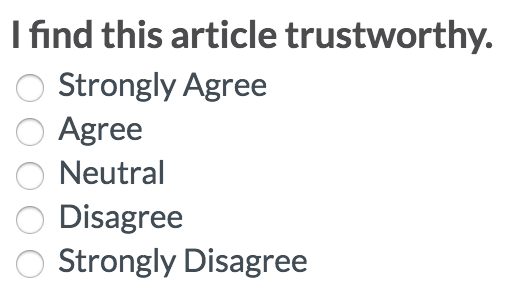
\includegraphics[width=.7\textwidth]{trust}  
%   \caption{Overall Trust Ratings
%     \label{fig:trust}}
% \end{figure}

\newpage
\begin{figure}[h!] 
\centering 
  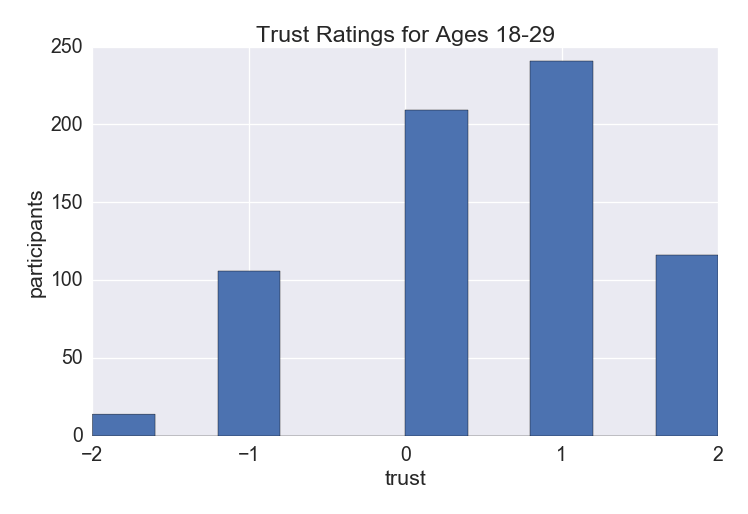
\includegraphics[width=0.8\textwidth]{trust_18-29} 
  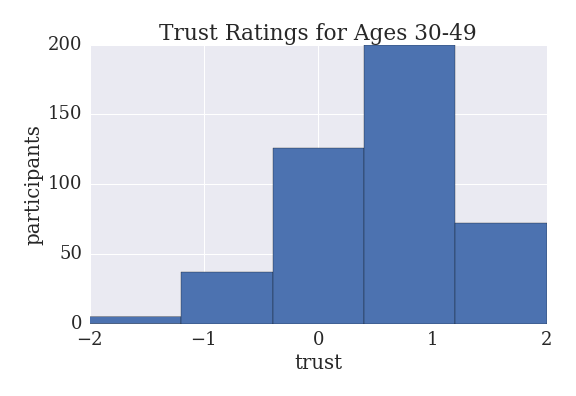
\includegraphics[width=0.8\textwidth]{trust_30-49} 
  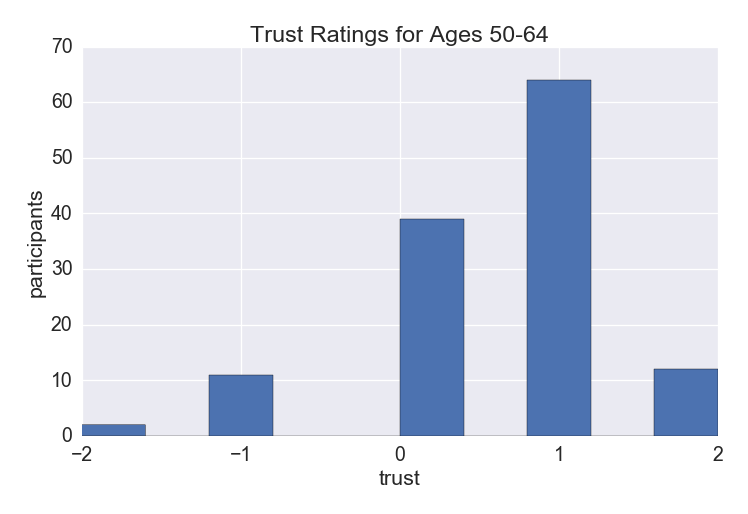
\includegraphics[width=0.8\textwidth]{trust_50-64} 
  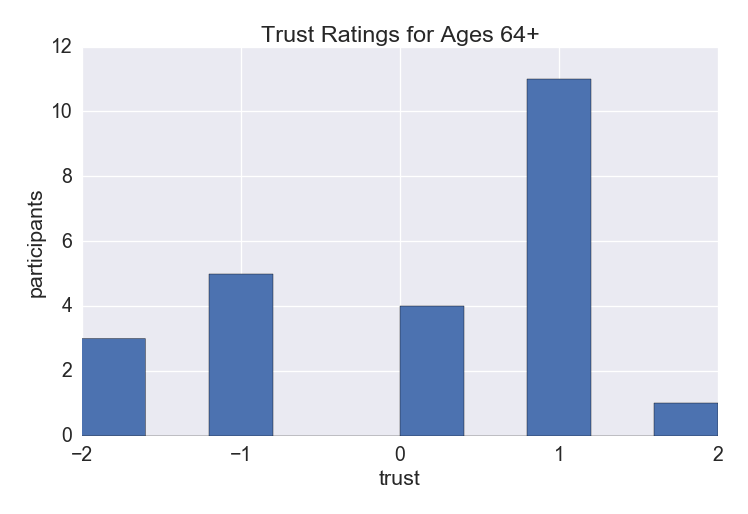
\includegraphics[width=0.8\textwidth]{trust_64+} 
  %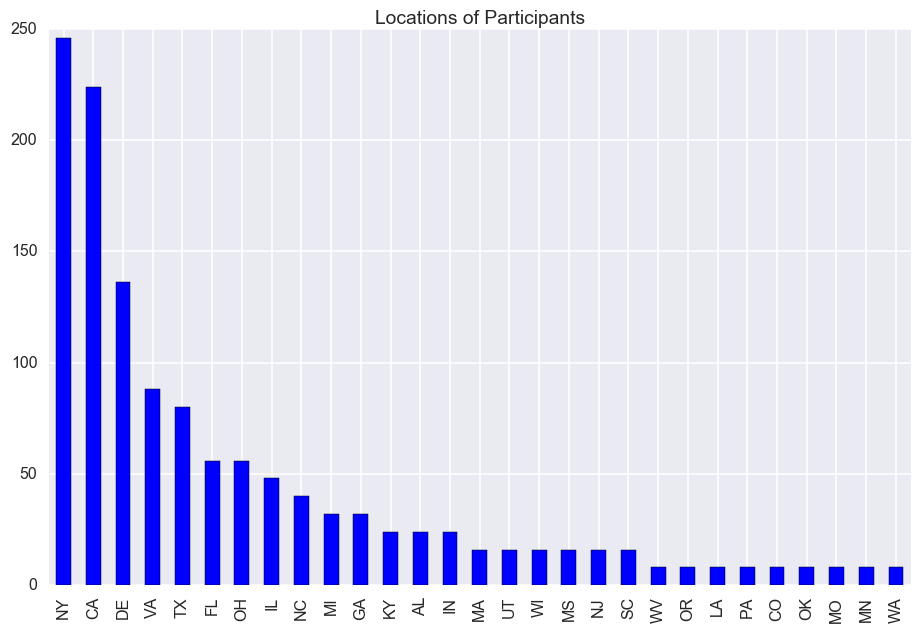
\includegraphics[width=0.32\textwidth]{location_study2} 
  \caption{Trust in Stories by Age Group
    \label{fig:trust-by-age}}
\end{figure}


% \begin{figure}[h!]  
% \centering 
%   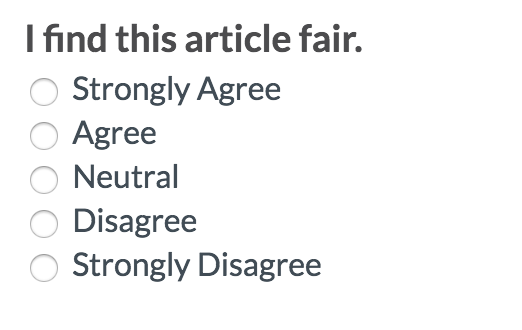
\includegraphics[width=.7\textwidth]{fair}  
%   \caption{Overall Fairness Ratings
%     \label{fig:fair}}
% \end{figure}

\newpage

% \begin{figure}[h!]  
% \centering  
%   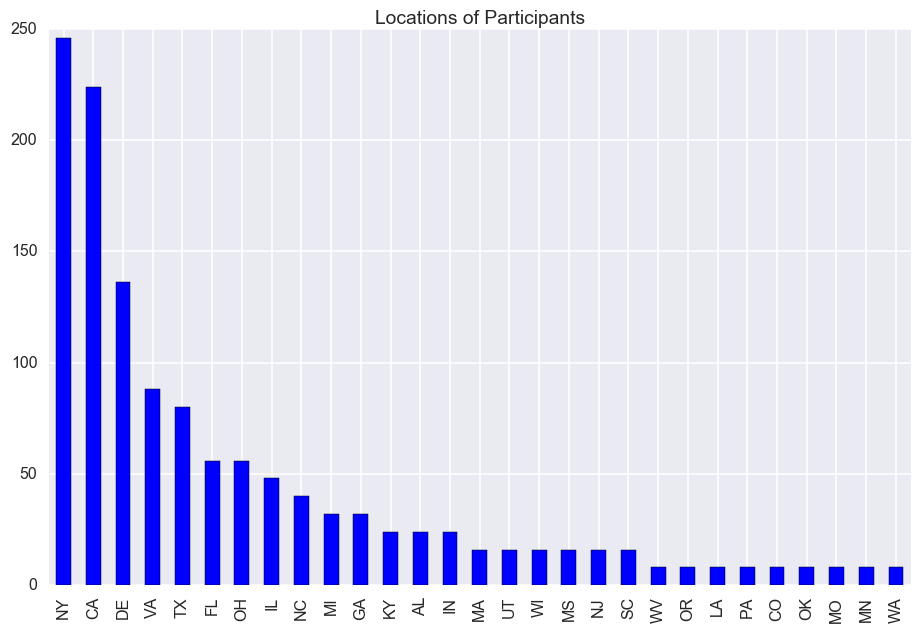
\includegraphics[width=0.9\textwidth]{location_study2} 
%   \caption{Locations of Participants
%     \label{fig:locations2}}
% \end{figure}

% \begin{figure}[h!]  
% \centering 
%   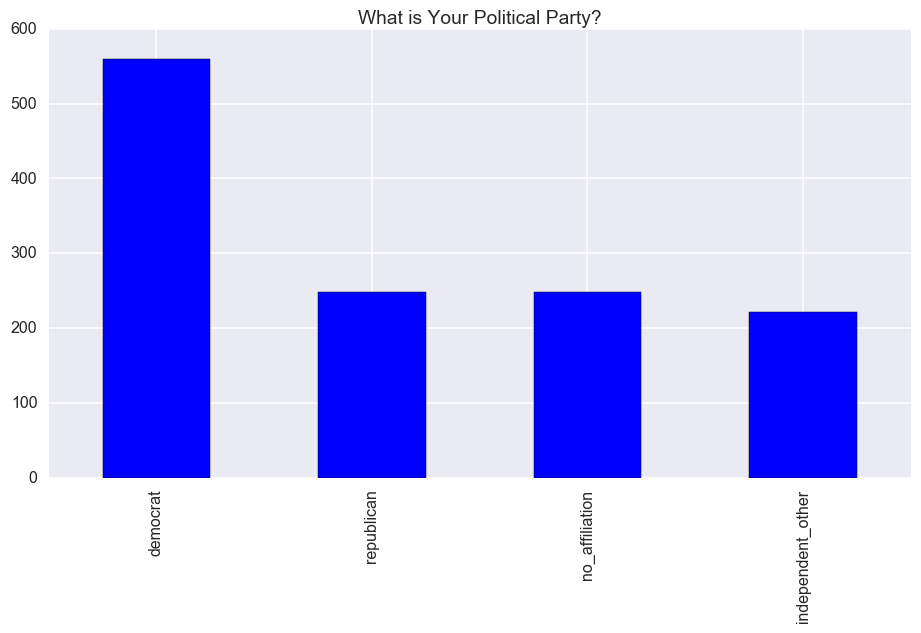
\includegraphics[width=.8\textwidth]{party_study2} 
%   \includegraphics[width=.8\textwidth]{voting_for_study2} 
%   %\includegraphics[width=0.32\textwidth]{location_study2} 
%   \caption{Political Affiliations of Participants
%     \label{fig:political2}}
% \end{figure}


% \begin{figure}[h!] 
% \label{fig:topics}
% \centering 
%   \includegraphics[width=0.45\textwidth]{trump_topics} 
%   \includegraphics[width=0.45\textwidth]{clinton_topics} 
%   \includegraphics[width=0.45\textwidth]{sanders_topics} 
%   \includegraphics[width=0.45\textwidth]{cruz_topics} 
%   \caption{Topic Distributions for Candidates}
% \end{figure}
% \clearpage
% \newpage
%  
%% This defines the bibliography file (main.bib) and the bibliography style.
%% If you want to create a bibliography file by hand, change the contents of
%% this file to a `thebibliography' environment.  For more information 
%% see section 4.3 of the LaTeX manual.
\begin{singlespace}
\bibliography{main}
\bibliographystyle{plain}
\end{singlespace}

\end{document}

